% Template adapted from https://github.com/jgm/pandoc-templates/blob/master/default.latex
% To be used with XeLaTex in memoiR
%%%%%%%%%%%%%%%%%%%%%%%%%%%%%%%%%%%%%%%%%%%%%%%%%%%%%%%%%%%%%%%%%%%%%%%%%%%%%%%%%%%%%%%%%

% Options for packages loaded elsewhere
\PassOptionsToPackage{unicode=true}{hyperref}
\PassOptionsToPackage{hyphens}{url}
\PassOptionsToPackage{dvipsnames,svgnames*,x11names*}{xcolor}
% Right to left support


\documentclass[
  10pt,
  italian,
  a4paper,
  extrafontsizes,onecolumn,openright
  ]{memoir}

% Double (or whatever) spacing

% Math
\usepackage{amssymb, amsmath}
% mathspec: arbitrary math fonts
\usepackage{unicode-math}
\defaultfontfeatures{Scale=MatchLowercase}
\defaultfontfeatures[\rmfamily]{Ligatures=TeX,Scale=1}

% Fonts
\usepackage{lmodern}
\usepackage{fontspec}

% Main font
% Specific sanserif font
% Specific monotype font
\setmonofont[Scale=0.85]{Inconsolata}
% Specific math font
% Chinese, Japanese, Corean fonts

% Use upquote for straight quotes in verbatim environments
\usepackage{upquote}
% Use microtype
\usepackage[]{microtype}
\UseMicrotypeSet[protrusion]{basicmath} % disable protrusion for tt fonts

% Verbatim in note

% Color links
\usepackage{xcolor}

% Strikeout

% Necessary for code chunks
\usepackage{color}
\usepackage{fancyvrb}
\newcommand{\VerbBar}{|}
\newcommand{\VERB}{\Verb[commandchars=\\\{\}]}
\DefineVerbatimEnvironment{Highlighting}{Verbatim}{commandchars=\\\{\}}
% Add ',fontsize=\small' for more characters per line
\usepackage{framed}
\definecolor{shadecolor}{RGB}{248,248,248}
\newenvironment{Shaded}{\begin{snugshade}}{\end{snugshade}}
\newcommand{\AlertTok}[1]{\textcolor[rgb]{0.94,0.16,0.16}{#1}}
\newcommand{\AnnotationTok}[1]{\textcolor[rgb]{0.56,0.35,0.01}{\textbf{\textit{#1}}}}
\newcommand{\AttributeTok}[1]{\textcolor[rgb]{0.77,0.63,0.00}{#1}}
\newcommand{\BaseNTok}[1]{\textcolor[rgb]{0.00,0.00,0.81}{#1}}
\newcommand{\BuiltInTok}[1]{#1}
\newcommand{\CharTok}[1]{\textcolor[rgb]{0.31,0.60,0.02}{#1}}
\newcommand{\CommentTok}[1]{\textcolor[rgb]{0.56,0.35,0.01}{\textit{#1}}}
\newcommand{\CommentVarTok}[1]{\textcolor[rgb]{0.56,0.35,0.01}{\textbf{\textit{#1}}}}
\newcommand{\ConstantTok}[1]{\textcolor[rgb]{0.00,0.00,0.00}{#1}}
\newcommand{\ControlFlowTok}[1]{\textcolor[rgb]{0.13,0.29,0.53}{\textbf{#1}}}
\newcommand{\DataTypeTok}[1]{\textcolor[rgb]{0.13,0.29,0.53}{#1}}
\newcommand{\DecValTok}[1]{\textcolor[rgb]{0.00,0.00,0.81}{#1}}
\newcommand{\DocumentationTok}[1]{\textcolor[rgb]{0.56,0.35,0.01}{\textbf{\textit{#1}}}}
\newcommand{\ErrorTok}[1]{\textcolor[rgb]{0.64,0.00,0.00}{\textbf{#1}}}
\newcommand{\ExtensionTok}[1]{#1}
\newcommand{\FloatTok}[1]{\textcolor[rgb]{0.00,0.00,0.81}{#1}}
\newcommand{\FunctionTok}[1]{\textcolor[rgb]{0.00,0.00,0.00}{#1}}
\newcommand{\ImportTok}[1]{#1}
\newcommand{\InformationTok}[1]{\textcolor[rgb]{0.56,0.35,0.01}{\textbf{\textit{#1}}}}
\newcommand{\KeywordTok}[1]{\textcolor[rgb]{0.13,0.29,0.53}{\textbf{#1}}}
\newcommand{\NormalTok}[1]{#1}
\newcommand{\OperatorTok}[1]{\textcolor[rgb]{0.81,0.36,0.00}{\textbf{#1}}}
\newcommand{\OtherTok}[1]{\textcolor[rgb]{0.56,0.35,0.01}{#1}}
\newcommand{\PreprocessorTok}[1]{\textcolor[rgb]{0.56,0.35,0.01}{\textit{#1}}}
\newcommand{\RegionMarkerTok}[1]{#1}
\newcommand{\SpecialCharTok}[1]{\textcolor[rgb]{0.00,0.00,0.00}{#1}}
\newcommand{\SpecialStringTok}[1]{\textcolor[rgb]{0.31,0.60,0.02}{#1}}
\newcommand{\StringTok}[1]{\textcolor[rgb]{0.31,0.60,0.02}{#1}}
\newcommand{\VariableTok}[1]{\textcolor[rgb]{0.00,0.00,0.00}{#1}}
\newcommand{\VerbatimStringTok}[1]{\textcolor[rgb]{0.31,0.60,0.02}{#1}}
\newcommand{\WarningTok}[1]{\textcolor[rgb]{0.56,0.35,0.01}{\textbf{\textit{#1}}}}

% Listings package

% Tables
\usepackage{longtable,booktabs,tabu}
% Fix footnotes in tables (requires footnote package)
\IfFileExists{footnote.sty}{\usepackage{footnote}\makesavenoteenv{longtable}}{}

% Graphics
\usepackage{graphicx,grffile}
\graphicspath{{images/}}
\makeatletter
\def\maxwidth{\ifdim\Gin@nat@width>\linewidth\linewidth\else\Gin@nat@width\fi}
\def\maxheight{\ifdim\Gin@nat@height>\textheight\textheight\else\Gin@nat@height\fi}
\makeatother
% Scale images if necessary, so that they will not overflow the page
% margins by default, and it is still possible to overwrite the defaults
% using explicit options in \includegraphics[width, height, ...]{}
\setkeys{Gin}{width=\maxwidth,height=\maxheight,keepaspectratio}

% Prevent overfull lines
\setlength{\emergencystretch}{3em}  
\providecommand{\tightlist}{%
  \setlength{\itemsep}{0pt}\setlength{\parskip}{0pt}}

% Number sections for memoir (secnumdepth counter is ignored)
\setsecnumdepth{section}

% Set default figure placement to htbp
\makeatletter
\def\fps@figure{htbp}
\makeatother

% Spacing in lists
\usepackage{enumitem}

% Polyglossia
\usepackage{polyglossia}
\setmainlanguage{it}
\setotherlanguage{en-US}

% BibLaTeX
\usepackage[backend=biber,style=authoryear-ibid,isbn=false,backref=true,giveninits=true,uniquename=init,maxcitenames=2,maxbibnames=150,sorting=nyt,sortcites=false,style=apa]{biblatex}
\addbibresource{refs.bib}

% cslreferences environment required by pandoc > 2.7



%%%%%%%%%%%%%%%%%%%%%%%%%%%%%%%%%%%%%%%%%%%%%%%%%%%%%%%%%%
% memoiR format

% Chapter Summary environment 
\usepackage[tikz]{bclogo}
\newenvironment{Summary}
  {\begin{bclogo}[logo=\bctrombone, noborder=true, couleur=lightgray!50]{In breve}\parindent0pt}
  {\end{bclogo}}
% Syntax:
%
%```{block, type='Summary'}
% Deliver message here.
% ```

% scriptsize code 
\let\oldverbatim\verbatim
\def\verbatim{\oldverbatim\scriptsize}
% Applies to code blocks and R code results
% code chunk options size='scriptsize' applies only to R code and results
% if the code chunk sets a different size, \def\verbatim{...} is prioritary for code results 


% Layout
%%%%%%%%%%%%%%%%%%%%%%%%%%%%%%%%%%%%%%%%%%%%%%%%%%%%%%%%%%

% Based on memoir, style companion
\newcommand{\MemoirChapStyle}{daleif1}
\newcommand{\MemoirPageStyle}{Ruled}

% Space between paragraphs
\usepackage{parskip}
  \abnormalparskip{3pt}

% Adjust margin paragraphs vertical position
\usepackage{marginfix}


% Margins
%%%%%%%%%%%%%%%%%%%%%%%%%%%%%%%%%%%%%%%

% allow use of '-',+','/' ans '*' to make simple length computation
\usepackage{calc}

% Full-width figures utilities
\newlength\widthw % full width
\newlength{\rf}
\newcommand*{\definesHSpace}{
  \strictpagecheck % slower but efficient detection of odd/even pages
  \checkoddpage
  \ifoddpage
  \setlength{\rf}{0mm}
  \else
  \setlength{\rf}{\marginparsep+\marginparwidth}
  \fi
}

\makeatletter
% 1" margins for the front matter.
\newcommand*{\SmallMargins}{
  \setlrmarginsandblock{1.5in}{1.5in}{*}
  \setmarginnotes{0.1in}{0.1in}{0.1in}
 \setulmarginsandblock{1.5in}{1in}{*}
  \checkandfixthelayout
  \ch@ngetext
  \clearpage
  \setlength{\widthw}{\textwidth+\marginparsep+\marginparwidth}
  \footnotesatfoot
  \chapterstyle{\MemoirChapStyle}  % Chapter and page styles must be recalled
  \pagestyle{\MemoirPageStyle}
}

% 3" outer margin for the main matter
\newcommand{\LargeMargins}{\SmallMargins}
\makeatother

% Figure captions and footnotes in outer margins


% Main title page with filigrane
%%%%%%%%%%%%%%%%%%%%%%%%%%%%%%%%%%%%%%%%%%%%%%%%%%%%%%%%%%

% Text blocks
\usepackage[absolute,overlay]{textpos}
  \setlength{\TPHorizModule}{1mm}
  \setlength{\TPVertModule}{1mm}

\newcommand{\MainTitlePage}[2]{
  \SmallMargins % Margins
  \pagestyle{empty} % No header/footer
  \textblockorigin{\stockwidth-\paperwidth-\trimedge}{\trimtop} % recto
  \begin{textblock*}{2mm}(\spinemargin/2,\uppermargin/2)
    \rule{1pt}{\paperheight-\uppermargin}
  \end{textblock*}
  \begin{textblock*}{\paperwidth*2/3}(\paperwidth/5, \paperheight/5)
    \flushright
    \begin{Spacing}{3}
      {\fontfamily{qtm}\selectfont\fontsize{45}{45}\selectfont\textsc{\thetitle}}
    \end{Spacing}
  \end{textblock*}
    \begin{textblock*}{\paperwidth*2/3}(\paperwidth/5, \paperheight/2)
    \flushright
    {\fontfamily{qtm}\huge\theauthor}
  \end{textblock*}
    \begin{textblock*}{\paperwidth*2/3}[0, 1](\spinemargin, \uppermargin+\textheight)
    \normalfont\thedate
  \end{textblock*}
  ~\\ % Print a character or the page will not exist
  \newpage
  \textblockorigin{\trimedge}{\trimtop} % verso
  \begin{textblock*}{\textwidth}(\paperwidth-\spinemargin-\textwidth, \uppermargin)
    #1
  \end{textblock*}
  \begin{textblock*}{\textwidth}[0,1](\paperwidth-\spinemargin-\textwidth, \uppermargin+\textheight+\footskip)
    \centering
    
\includegraphics[width=\paperwidth/4]{logo}\\ \bigskip
    #2
  \end{textblock*}
  ~\\ % Print a character or the page will not exist
  \newpage
}

% Clear page and open an even one (\clearpage opens an odd one)
\newcommand{\evenpage}{
  \clearpage
  \strictpagecheck % slower but efficient detection of odd/even pages
  \checkoddpage
  \ifoddpage
    \thispagestyle{empty}
    ~\\ % Print a character or the page will not exist
    \newpage
  \else
    % do nothing
  \fi
}


%% PDF title page to insert
%%%%%%%%%%%%%%%%%%%%%%%%%%%%%%%%%%%%%%%%%%%%%%%%%%%%%%%%%%



%% Bibliography
%%%%%%%%%%%%%%%%%%%%%%%%%%%%%%%%%%%%%%%%%%%%%%%%%%%%%%%%%%

\usepackage[strict,autostyle]{csquotes}
% Repeated citation as author-year-title instead of author-title (modification of footcite:note in verbose-inote.cbx)

%% Table of Contents
%%%%%%%%%%%%%%%%%%%%%%%%%%%%%%%%%%%%%%%%%%%%%%%%%%%%%%%%%%

% fix the typesetting of the part number
\renewcommand\partnumberlinebox[2]{#2\ ---\ }


% Fonts
%%%%%%%%%%%%%%%%%%%%%%%%%%%%%%%%%%%%%%%%%%%%%%%%%%%%%%%%%%


% Hyperref comes last
%%%%%%%%%%%%%%%%%%%%%%%%%%%%%%%%%%%%%%%%%%%%%%%%%%%%%%%%%%

\usepackage{hyperref}
\hypersetup{
  pdftitle={Psicometria},
  pdfauthor={Corrado Caudek},
  colorlinks=true,
  linkcolor=Maroon,
  citecolor=Blue,
  urlcolor=Blue,
  breaklinks=true}

% Don't use monospace font for urls
\urlstyle{same}


% Title, author, date from YAML to LaTeX
%%%%%%%%%%%%%%%%%%%%%%%%%%%%%%%%%%%%%%%%%%%%%%%%%%%%%%%%%%

\title{Psicometria}

\author{Corrado Caudek}

\date{2021-11-28}


% Include headers (preamble.tex) here
%%%%%%%%%%%%%%%%%%%%%%%%%%%%%%%%%%%%%%%%%%%%%%%%%%%%%%%%%%
% Add LaTeX code into the preamble of the document here
\hyphenation{bio-di-ver-si-ty sap-lings}


%%%%%%%%%%%%%%%%%%%%%%%%%%%%%%%%%%%%%%%%%%%%%%%%%%%%%%%%%%%%%%%%%%%%%%%%%
% memoiR dalef3 chapter style 
% https://ctan.crest.fr/tex-archive/info/latex-samples/MemoirChapStyles/MemoirChapStyles.pdf
\usepackage{soul}
\definecolor{nicered}{rgb}{.647,.129,.149}
\makeatletter
\newlength\dlf@normtxtw
\setlength\dlf@normtxtw{\textwidth}
\def\myhelvetfont{\def\sfdefault{mdput}}
\newsavebox{\feline@chapter}
\newcommand\feline@chapter@marker[1][4cm]{%
  \sbox\feline@chapter{%
    \resizebox{!}{#1}{\fboxsep=1pt%
	  \colorbox{nicered}{\color{white}\bfseries\sffamily\thechapter}%
	}}%
  \rotatebox{90}{%
    \resizebox{%
	  \heightof{\usebox{\feline@chapter}}+\depthof{\usebox{\feline@chapter}}}%
	{!}{\scshape\so\@chapapp}}\quad%
  \raisebox{\depthof{\usebox{\feline@chapter}}}{\usebox{\feline@chapter}}%
 }
\newcommand\feline@chm[1][4cm]{%
  \sbox\feline@chapter{\feline@chapter@marker[#1]}%
  \makebox[0pt][l]{% aka \rlap
    \makebox[1cm][r]{\usebox\feline@chapter}%
  }}
\makechapterstyle{daleif1}{
  \renewcommand\chapnamefont{\normalfont\Large\scshape\raggedleft\so}
  \renewcommand\chaptitlefont{\normalfont\huge\bfseries\scshape\color{nicered}}
  \renewcommand\chapternamenum{}
  \renewcommand\printchaptername{}
  \renewcommand\printchapternum{\null\hfill\feline@chm[2.5cm]\par}
  \renewcommand\afterchapternum{\par\vskip\midchapskip}
  \renewcommand\printchaptertitle[1]{\chaptitlefont\raggedleft ##1\par}
}
\makeatother

\DeclareMathOperator{\Var}{Var} % Define variance operator
\DeclareMathOperator{\SD}{SD} % Define sd operator
\DeclareMathOperator{\Cov}{Cov} % Define covariance operator
\DeclareMathOperator{\Corr}{Corr} % Define correlation operator
\DeclareMathOperator{\Me}{Me} % Define mediane operator
\DeclareMathOperator{\Mo}{Mo} % Define mode operator
\DeclareMathOperator{\Bin}{Bin} % Define binomial operator
\DeclareMathOperator{\Bernoulli}{Bernoulli} % Define Bernoulli operator
\DeclareMathOperator{\Poi}{Poi} % Define Poisson operator
\DeclareMathOperator{\Uniform}{Uniform} % Define Uniform operator
\DeclareMathOperator{\Cauchy}{Cauchy} % Define Cauchy operator
\DeclareMathOperator{\elpd}{elpd} % Define elpd operator
\DeclareMathOperator{\lppd}{lppd} % Define lppd operator
\DeclareMathOperator{\LOO}{LOO} % Define LOO operator
\DeclareMathOperator{\B}{\mathscr{B}} % Define Bernoulli operator
\newcommand{\R}{\textsf{R}} % Define R programming language symbol
\newcommand{\E}{\mathbb{E}} % Define expected value operator
\newcommand{\Real}{\mathbb{R}} % Define real number operator
\newcommand{\Prob}{\mathscr{P}}
\DeclareMathOperator*{\argmin}{arg\,min} % thin space, limits on side in displays
\DeclareMathOperator*{\argmax}{arg\,max} % thin space, limits on side in displays

\raggedbottom % allow variable (ragged) site heights
\frenchspacing

\usepackage[
  labelfont=bf, 
  font={small, it} 
]{caption} 
\usepackage{upquote} % print correct quotes in verbatim-environments
\usepackage{empheq} 
\usepackage{xfrac}




\usepackage{booktabs}
\usepackage{longtable}
\usepackage{array}
\usepackage{multirow}
\usepackage{wrapfig}
\usepackage{float}
\usepackage{colortbl}
\usepackage{pdflscape}
\usepackage{tabu}
\usepackage{threeparttable}
\usepackage{threeparttablex}
\usepackage[normalem]{ulem}
\usepackage{makecell}
\usepackage{xcolor}


% End of preamble
%%%%%%%%%%%%%%%%%%%%%%%%%%%%%%%%%%%%%%%%%%%%%%%%%%%%%%%%%%


\usepackage{amsthm}
\newtheorem{theorem}{Teorema}[chapter]
\newtheorem{lemma}{Lemma}[chapter]
\newtheorem{corollary}{Corollario}[chapter]
\newtheorem{proposition}{Proposizione}[chapter]
\newtheorem{conjecture}{Congettura}[chapter]
\theoremstyle{definition}
\newtheorem{definition}{Definizione}[chapter]
\theoremstyle{definition}
\newtheorem{example}{Esempio}[chapter]
\theoremstyle{definition}
\newtheorem{exercise}{Exercizio}[chapter]
\theoremstyle{definition}
\newtheorem{hypothesis}{Hypothesis}[chapter]
\theoremstyle{remark}
\newtheorem*{remark}{Osservazione}
\newtheorem*{solution}{Soluzione}
\begin{document}
\frontmatter

% Title page
%%%%%%%%%%%%%%%%%%%%%%%%%%%%%%%%%%%%%%%%%%%%%%%%%%%%%%%%%%


\MainTitlePage{Questo documento è stato realizzato con:

\begin{itemize}
  \item \LaTeX\; e la classe memoir (\url{http://www.ctan.org/pkg/memoir});
  \item $\R$ (\url{http://www.r-project.org/}) e RStudio (\url{http://www.rstudio.com/});
  \item bookdown (\url{http://bookdown.org/}) e memoiR (\url{https://ericmarcon.github.io/memoiR/}).
\end{itemize}}{Nel blog della mia pagina personale sono forniti alcuni approfondimenti degli argomenti qui trattati.

\url{https://ccaudek.github.io/caudeklab/}}


% Before Body
%%%%%%%%%%%%%%%%%%%%%%%%%%%%%%%%%%%%%%%%%%%%%%%%%%%%%%%%%%





% Contents
%%%%%%%%%%%%%%%%%%%%%%%%%%%%%%%%%%%%%%%%%%%%%%%%%%%%%%%%%%

\LargeMargins
{
\hypersetup{linkcolor=}
\setcounter{tocdepth}{2}
\tableofcontents
}


% Body
%%%%%%%%%%%%%%%%%%%%%%%%%%%%%%%%%%%%%%%%%%%%%%%%%%%%%%%%%%

\LargeMargins
\scriptsize

\normalsize

\chapter*{}

\vfill

\scriptsize

\normalsize

\scriptsize

Copyright \(\copyright\) 2022.

\normalsize

Data della versione presente: Novembre 28, 2021.

\hypertarget{prefazione}{%
\chapter{Prefazione}\label{prefazione}}

\textbf{Data Science per psicologi} contiene il materiale delle lezioni dell'insegnamento di \emph{Psicometria B000286} (A.A. 2021/2022) rivolto agli studenti del primo anno del Corso di Laurea in Scienze e Tecniche Psicologiche dell'Università degli Studi di Firenze.

L'insegnamento di Psicometria si propone di fornire agli studenti un'introduzione all'analisi dei dati in psicologia.
Le conoscenze/competenze che verranno sviluppate in questo insegnamento sono quelle della \emph{Data science}, ovvero le conoscenze/competenze che si pongono all'intersezione tra statistica (ovvero, richiedono la capacità di comprendere teoremi statistici) e informatica (ovvero, richiedono la capacità di sapere utilizzare un software).

\hypertarget{la-psicologia-e-la-data-science}{%
\section*{La psicologia e la Data Science}\label{la-psicologia-e-la-data-science}}
\addcontentsline{toc}{section}{La psicologia e la Data Science}

\begin{quote}
It's worth noting, before getting started, that this material is hard. If you find yourself confused at any point, you are normal. Any sense of confusion you feel is just your brain correctly calibrating to the subject matter. Over time, confusion is replaced by comprehension {[}\ldots{]} --- Richard McElreath
\end{quote}

Sembra sensato spendere due parole su un tema che è importante per gli studenti: quello indicato dal titolo di questo Capitolo. È ovvio che agli studenti di psicologia la statistica non piace. Se piacesse, forse studierebbero Data Science e non psicologia; ma non lo fanno. Di conseguenza, gli studenti di psicologia si chiedono: ``perché dobbiamo perdere tanto tempo a studiare queste cose quando in realtà quello che ci interessa è tutt'altro?'\,' Questa è una bella domanda.

C'è una ragione molto semplice che dovrebbe farci capire perché la Data Science è così importante per la psicologia. Infatti, a ben pensarci, la psicologia è una disciplina intrinsecamente statistica, se per statistica intendiamo quella disciplina che studia la variazione delle caratteristiche degli individui nella popolazione. La psicologia studia \emph{gli individui} ed è proprio la variabilità inter- e intra-individuale ciò che vogliamo descrivere e, in certi casi, predire. In questo senso, la psicologia è molto diversa dall'ingegneria, per esempio. Le proprietà di un determinato ponte sotto certe condizioni, ad esempio, sono molto simili a quelle di un altro ponte, sotto le medesime condizioni. Quindi, per un ingegnere la statistica è poco importante: le proprietà dei materiali sono unicamente dipendenti dalla loro composizione e restano costanti. Ma lo stesso non può dirsi degli individui: ogni individuo è unico e cambia nel tempo. E le variazioni tra gli individui, e di un individuo nel tempo, sono l'oggetto di studio proprio della psicologia: è dunque chiaro che i problemi che la psicologia si pone sono molto diversi da quelli affrontati, per esempio, dagli ingegneri. Questa è la ragione per cui abbiamo tanto bisogno della \emph{data science} in psicologia: perché la \emph{data science} ci consente di descrivere la variazione e il cambiamento. E queste sono appunto le caratteristiche di base dei fenomeni psicologici.

Sono sicuro che, leggendo queste righe, a molti studenti sarà venuta in mente la seguente domanda: perché non chiediamo a qualche esperto di fare il ``lavoro sporco'' (ovvero le analisi statistiche) per noi, mentre noi (gli psicologi) ci occupiamo solo di ciò che ci interessa, ovvero dei problemi psicologici slegati dai dettagli ``tecnici'' della \emph{data science}?
La risposta a questa domanda è che non è possibile progettare uno studio psicologico sensato senza avere almeno una comprensione rudimentale della \emph{data science}. Le tematiche della \emph{data science} non possono essere ignorate né dai ricercatori in psicologia né da coloro che svolgono la professione di psicologo al di fuori dell'Università. Infatti, anche i professionisti al di fuori dall'università non possono fare a meno di leggere la letteratura psicologica più recente: il continuo aggiornamento delle conoscenze è infatti richiesto dalla deontologia della professione. Ma per potere fare questo è necessario conoscere un bel po' di \emph{data science}! Basta aprire a caso una rivista specialistica di psicologia per rendersi conto di quanto ciò sia vero: gli articoli che riportano i risultati delle ricerche psicologiche sono zeppi di analisi statistiche e di modelli formali. E la comprensione della letteratura psicologica rappresenta un requisito minimo nel bagaglio professionale dello psicologo.

Le considerazioni precedenti cercano di chiarire il seguente punto: la \emph{data science} non è qualcosa da studiare a malincuore, in un singolo insegnamento universitario, per poi poterla tranquillamente dimenticare. Nel bene e nel male, gli psicologi usano gli strumenti della \emph{data science} in tantissimi ambiti della loro attività professionale: in particolare quando costruiscono, somministrano e interpretano i test psicometrici. È dunque chiaro che possedere delle solide basi di \emph{data science} è un tassello imprescindibile del bagaglio professionale dello psicologo. In questo insegnamento verrano trattati i temi base della \emph{data science} e verrà adottato un punto di vista bayesiano, che corrisponde all'approccio più recente e sempre più diffuso in psicologia.

\hypertarget{come-studiare}{%
\section*{Come studiare}\label{come-studiare}}
\addcontentsline{toc}{section}{Come studiare}

\begin{quote}
I know quite certainly that I myself have no special talent. Curiosity, obsession and dogged endurance, combined with self-criticism, have brought me to my ideas. --- Albert Einstein
\end{quote}

Il giusto metodo di studio per prepararsi all'esame di Psicometria è quello di seguire attivamente le lezioni, assimilare i concetti via via che essi vengono presentati e verificare in autonomia le procedure presentate a lezione. Incoraggio gli studenti a farmi domande per chiarire ciò che non è stato capito appieno. Incoraggio gli studenti a utilizzare i forum attivi su Moodle e, soprattutto, a svolgere gli esercizi proposti su Moodle. I problemi forniti su Moodle rappresentano il livello di difficoltà richiesto per superare l'esame e consentono allo studente di comprendere se le competenze sviluppate fino a quel punto sono sufficienti rispetto alle richieste dell'esame.

La prima fase dello studio, che è sicuramente individuale, è quella in cui è necessario acquisire le conoscenze teoriche relative ai problemi che saranno presentati all'esame. La seconda fase di studio, che può essere facilitata da scambi con altri e da incontri di gruppo, porta ad acquisire la capacità di applicare le conoscenze: è necessario capire come usare un software (\R) per applicare i concetti statistici alla specifica situazione del problema che si vuole risolvere. Le due fasi non sono però separate: il saper fare molto spesso ci aiuta a capire meglio.

\hypertarget{sviluppare-un-metodo-di-studio-efficace}{%
\section*{Sviluppare un metodo di studio efficace}\label{sviluppare-un-metodo-di-studio-efficace}}
\addcontentsline{toc}{section}{Sviluppare un metodo di studio efficace}

\begin{quote}
Memorization is not learning. --- Richard Phillips Feynman
\end{quote}

Avendo insegnato molte volte in passato un corso introduttivo di analisi dei dati ho notato nel corso degli anni che gli studenti con l'atteggiamento mentale che descriverò qui sotto generalmente ottengono ottimi risultati. Alcuni studenti sviluppano naturalmente questo approccio allo studio, ma altri hanno bisogno di fare uno sforzo per maturarlo. Fornisco qui sotto una breve descrizione del ``metodo di studio'\,' che, nella mia esperienza, è il più efficace per affrontare le richieste di questo insegnamento \autocite{burger20125}.

\begin{itemize}
\tightlist
\item
  Dedicate un tempo sufficiente al materiale di base, apparentemente facile; assicuratevi di averlo capito bene. Cercate le lacune nella vostra comprensione. Leggere presentazioni diverse dello stesso materiale (in libri o articoli diversi) può fornire nuove intuizioni.
\end{itemize}

\begin{itemize}
\item
  Gli errori che facciamo sono i nostri migliori maestri. Istintivamente cerchiamo di dimenticare subito i nostri errori. Ma il miglior modo di imparare è apprendere dagli errori che commettiamo. In questo senso, una soluzione corretta è meno utile di una soluzione sbagliata. Quando commettiamo un errore questo ci fornisce un'informazione importante: ci fa capire qual è il materiale di studio sul quale dobbiamo ritornare e che dobbiamo capire meglio.
\item
  C'è ovviamente un aspetto ``psicologico'' nello studio. Quando un esercizio o problema ci sembra incomprensibile, la cosa migliore da fare è dire: ``mi arrendo'', ``non ho idea di cosa fare!''. Questo ci rilassa: ci siamo già arresi, quindi non abbiamo niente da perdere, non dobbiamo più preoccuparci. Ma non dobbiamo fermarci qui. Le cose ``migliori'' che faccio (se ci sono) le faccio quando non ho voglia di lavorare. Alle volte, quando c'è qualcosa che non so fare e non ho idea di come affontare, mi dico: ``oggi non ho proprio voglia di fare fatica'', non ho voglia di mettermi nello stato mentale per cui ``in 10 minuti devo risolvere il problema perché dopo devo fare altre cose''. Però ho voglia di \emph{divertirmi} con quel problema e allora mi dedico a qualche aspetto ``marginale'' del problema, che so come affrontare, oppure considero l'aspetto più difficile del problema, quello che non so come risolvere, ma invece di cercare di risolverlo, guardo come altre persone hanno affrontato problemi simili, opppure lo stesso problema in un altro contesto. Non mi pongo l'obiettivo ``risolvi il problema in 10 minuti'', ma invece quello di farmi un'idea ``generale'' del problema, o quello di capire un caso più specifico e più semplice del problema. Senza nessuna pressione. Infatti, in quel momento ho deciso di non lavorare (ovvero, di non fare fatica). Va benissimo se ``parto per la tangente'', ovvero se mi metto a leggere del materiale che sembra avere poco a che fare con il problema centrale (le nostre intuizioni e la nostra curiosità solitamente ci indirizzano sulla strada giusta). Quando faccio così, molto spesso trovo la soluzione del problema che mi ero posto e, paradossalmente, la trovo in un tempo minore di quello che, in precedenza, avevo dedicato a ``lavorare'' al problema. Allora perché non faccio sempre così? C'è ovviamente l'aspetto dei ``10 minuti'' che non è sempre facile da dimenticare. Sotto pressione, possiamo solo agire in maniera automatica, ovvero possiamo solo applicare qualcosa che già sappiamo fare. Ma se dobbiamo imparare qualcosa di nuovo, la pressione è un impedimento.
\item
  È utile farsi da soli delle domande sugli argomenti trattati, senza limitarsi a cercare di risolvere gli esercizi che vengono assegnati. Quando studio qualcosa mi viene in mente: ``se questo è vero, allora deve succedere quest'altra cosa''. Allora verifico se questo è vero, di solito con una simulazione. Se i risultati della simulazione sono quelli che mi aspetto, allora vuol dire che ho capito. Se i risultati sono diversi da quelli che mi aspettavo, allora mi rendo conto di non avere capito e ritorno indietro a studiare con più attenzione la teoria che pensavo di avere capito -- e ovviamente mi rendo conto che c'era un aspetto che avevo frainteso. Questo tipo di verifica è qualcosa che dobbiamo fare da soli, in prima persona: nessun altro può fare questo al posto nostro.
\item
  Non aspettatevi di capire tutto la prima volta che incontrate un argomento nuovo.\footnote{Ricordatevi inoltre che gli individui tendono a sottostimare la propria capacità di apprendere \autocite{horn2021underestimating}.} È utile farsi una nota mentalmente delle lacune nella vostra comprensione e tornare su di esse in seguito per carcare di colmarle. L'atteggiamento naturale, quando non capiamo i dettagli di qualcosa, è quello di pensare: ``non importa, ho capito in maniera approssimativa questo punto, non devo preoccuparmi del resto''. Ma in realtà non è vero: se la nostra comprensione è superficiale, quando il problema verrà presentato in una nuova forma, non riusciremo a risolverlo. Per cui i dubbi che ci vengono quando studiamo qualcosa sono il nostro alleato più prezioso: ci dicono esattamente quali sono gli aspetti che dobbiamo approfondire per potere migliorare la nostra preparazione.
\item
  È utile sviluppare una visione d'insieme degli argomenti trattati, capire l'obiettivo generale che si vuole raggiungere e avere chiaro il contributo che i vari pezzi di informazione forniscono al raggiungimento di tale obiettivo. Questa organizzazione mentale del materiale di studio facilita la comprensione. È estremamente utile creare degli schemi di ciò che si sta studiando. Non aspettate che sia io a fornirvi un riepilogo di ciò che dovete imparare: sviluppate da soli tali schemi e tali riassunti.
\item
  Tutti noi dobbiamo imparare l'arte di trovare le informazioni, non solo nel caso di questo insegnamento. Quando vi trovate di fronte a qualcosa che non capite, o ottenete un oscuro messaggio di errore da un software, ricordatevi: ``Google is your friend''.
\end{itemize}

\bigskip

Corrado Caudek

\bigskip

Febbraio 2022

\mainmatter

\hypertarget{part-statistica-descrittiva-ed-analisi-esplorativa-dei-dati}{%
\part*{Statistica descrittiva ed analisi esplorativa dei dati}\label{part-statistica-descrittiva-ed-analisi-esplorativa-dei-dati}}
\addcontentsline{toc}{part}{Statistica descrittiva ed analisi esplorativa dei dati}

\hypertarget{descriptive-stats}{%
\chapter{Statistica descrittiva}\label{descriptive-stats}}

\begin{Summary}
Le analisi esplorative dei dati e la statistica descrittiva
costituiscono la prima fase dell'analisi dei dati psicologici.
Consentono di capire come i dati sono distribuiti, ci aiutano ad
individuare le osservazioni anomale e gli errori di tabulazione.
Consentono di visualizzare e di studiare le relazioni tra le variabili.
\end{Summary}

\hypertarget{chapter-descript}{%
\section{Introduzione all'esplorazione dei dati}\label{chapter-descript}}

Le analisi esplorative dei datisono indispensabili per condurre in modo corretto una qualsiasi analisi statistica, dal livello base a quello avanzato. Si parla di analisi descrittiva se l'obiettivo è quello di descrivere le caratteristiche di un campione. Si parla di analisi esplorativa dei dati (\emph{Exploratory Data Analysis} o EDA) se l'obiettivo è quello di esplorare i dati alla ricerca di nuove informazioni e relazioni tra variabili. Questa distinzione, seppur importante a livello teorico, nella pratica è più fumosa perché spesso entrambe le situazioni si verificano contemporaneamente nella stessa indagine statistica e le metodologie di analisi che si utilizzano sono molto simili.

Né il calcolo delle statistiche descrittive né l'analisi esplorativa dei dati possono essere condotte senza utilizzare un software. Le descrizioni dei concetti di base della EDA saranno dunque fornite di pari passo alla spiegazione di come le quantità discusse possono essere calcolate in pratica utilizzando R.

\hypertarget{un-excursus-storico}{%
\section{Un excursus storico}\label{un-excursus-storico}}

Nel 1907 Francis Galton, cugino di Charles Darwin, matematico e
statistico autodidatta, geografo, esploratore, teorico della
dattiloscopia (ovvero, dell'uso delle impronte digitali a fini
identificativi) e dell'eugenetica, scrisse una lettera alla rivista
scientifica Nature sulla sua visita alla \emph{Fat Stock and Poultry
Exhibition} di Plymouth. Lì vide alcuni membri del pubblico partecipare
ad un gioco il cui scopo era quello di indovinare il peso della carcassa
di un grande bue che era appena stato scuoiato. Galton si procurò i 787
dei biglietti che erano stati compilati dal pubblico e considerò il
valore medio di 547 kg come la ``scelta democratica'' dei partecipanti, in
quanto ``ogni altra stima era stata giudicata troppo alta o troppo bassa
dalla maggioranza dei votanti''. Il punto interessante è che il peso
corretto di 543 kg si dimostrò essere molto simile alla ``scelta
democratica'' basata sulle stime dei 787 partecipanti. Galton intitolò la
sua lettera a Nature \emph{Vox Populi} (voce del popolo), ma questo processo
decisionale è ora meglio conosciuto come la ``saggezza delle folle''
(\emph{wisdom of crowds}). Possiamo dire che, nel suo articolo del 1907,
Galton effettuò quello che ora chiamiamo un riepilogo dei dati, ovvero
calcolò un indice sintetico a partire da un insieme di dati. In questo
capitolo esamineremo le tecniche che sono state sviluppate nel secolo
successivo per riassumere le grandi masse di dati con cui sempre più
spesso ci dobbiamo confrontare. Vedremo come calcolare e interpretare
gli indici di posizione e di dispersione, discuteremo le distribuzioni
di frequenze e le relazioni tra variabili. Vedremo inoltre quali sono le
tecniche di visualizzazione che ci consentono di rappresentare questi
sommari dei dati mediante dei grafici. Ma prima di entrare nei dettagli, prendiamoci un momento per capire perché abbiamo bisogno della statistica e, per ciò che stiamo discutendo qui, della statistica descrittiva.

In generale, che cos'è la statistica? Ci sono molte definizioni. Fondamentalmente, la statistica è un insieme di tecniche che ci consentono di dare un senso al mondo attraverso i dati. Ciò avviene tramite il processo di analisi statistica. L'analisi statistica traduce le domande che abbiamo a proposito del mondo in modelli matematici, utilizza i dati per scegliere i modelli matematici che sono apppropriati per descrivere il mondo e, infine, applica tali modelli per trovare una risposta alle domande che ci siamo posti. La statistica consente quindi di collegare le nostre domande a proposito del mondo ai dati, di utilizzare i dati per trovare le risposte alle domande che ci siamo posti e di valutare l'impatto delle risposte che abbiamo trovato.

\hypertarget{riassumere-i-dati}{%
\section{Riassumere i dati}\label{riassumere-i-dati}}

Iniziamo a porci una domanda. Quando riassumiamo i dati, necessariamente buttiamo via delle informazioni; ma è una buona idea procedere in questo modo? Non sarebbe meglio conservare le informazioni specifiche di ciascun soggetto che partecipa ad un esperimento psicologico, al di là di ciò che viene trasmesso dagli indici riassuntivi della statistica descrittiva? Che dire delle informazioni che descrivono come sono stati raccolti i dati, come l'ora del giorno o l'umore del partecipante? Tutte queste informazioni vengono perdute quando riassumiamo i dati. La risposta alla domanda che ci siamo posti è che, in generale, non è una buona idea conservare tutti i dettagli di ciò che sappiamo. È molto più utile riassumere le informazioni perché la semplificazione risultante consente i processi di \emph{generalizzazione}.

In un contesto letterario, l'importanza della generalizzazione è stata
sottolineata da Jorge Luis Borges nel suo racconto ``Funes o della
memoria'', che descrive un individuo che perde la capacità di
dimenticare. Borges si concentra sulla relazione tra generalizzazione e
pensiero:

\begin{quote}
Pensare è dimenticare una differenza, generalizzare, astrarre. Nel mondo troppo pieno di Funes, c'erano solo dettagli.
\end{quote}

Come possiamo ben capire, la vita di Funes non è facile. Se facciamo
riferimento alla psicologia possiamo dire che gli psicologi hanno
studiato a lungo l'utilità della generalizzazione per il pensiero. Un
esempio è fornito dal fenomeno della formazione dei concetti e lo
psicologo che viene in mente a questo proposito è sicuramente Eleanor
Rosch, la quale ha studiato i principi di base della categorizzazione. I
concetti ci forniscono uno strumento potente per organizzare le
conoscenze. Noi siamo in grado di riconoscere facilmente i diversi
esemplare di un concetto -- per esempio, ``gli uccelli'' -- anche se i
singoli esemplari che fanno parte di una categoria sono molto diversi
tra loro (l'aquila, il gabbiano, il pettirosso). L'uso dei concetti, cioè
la generalizzazione, è utile perché ci consente di fare previsioni sulle
proprietà dei singoli esemplari che appartengono ad una categoria, anche
se non abbiamo mai avuto esperienza diretta con essi -- per esempio,
possiamo fare la predizione che tutti gli uccelli possono volare e
mangiare vermi, ma non possono guidare un'automobile o parlare in
inglese. Queste previsioni non sono sempre corrette, ma sono utili.

Le statistiche descrittive, in un certo senso, ci fornisco l'analogo dei
``prototipi'' che, secondo Eleanor Rosch, stanno alla base del processo
psicologico di creazione dei concetti. Un prototipo è l'esemplare più
rappresentativo di una categoria. In maniera simile, una statistica
descrittiva come la media, ad esempio, potrebbe essere intesa come
l'osservazione ``tipica''.

La statistica descrittiva ci fornisce gli strumenti per riassumere i
dati che abbiamo a disposizione in una forma visiva o numerica. Le
rappresentazioni grafiche più usate della statistica descrittiva sono
gli istogrammi, i diagrammi a dispersione o i box-plot, e gli indici
sintetici più comuni sono la media, la mediana, la varianza e la
deviazione standard.

\hypertarget{distribuzioni-di-frequenze}{%
\section{Distribuzioni di frequenze}\label{distribuzioni-di-frequenze}}

Per introdurre i principali strumenti della statistica descrittiva considereremo qui i dati raccolti da \textcite{zetschefuture2019}\footnote{Si veda l'Appendice \ref{es-pratico-zetsche}.}. Questi autori hanno studiato le aspettative negative le quali sono state evidenziate come un meccanismo chiave nel mantenimento e nella reiterazione della depressione. \textcite{zetschefuture2019} hanno valutato le aspettative di individui depressi circa il loro umore futuro ed si sono chiesti se queste aspettative fossero accurate oppure distorte negativamente.

In uno degli studi descritti viene esaminato un campione costituito da 30 soggetti con almeno un episodio depressivo maggiore e da 37 controlli sani. Gli autori hanno misurato il livello depressivo con il \emph{Beck Depression Inventory} (BDI-II). Ma qual è la la gravità della depressione riportata dai soggetti nel campione esaminato da \textcite{zetschefuture2019}?

Per rispondere a questa domanda, iniziamo a leggere in \(\R\) i dati, assumendo che il file \texttt{data.mood.csv} si trovi nella cartella \texttt{data} contenuta nella \emph{working directory}.

\begin{Shaded}
\begin{Highlighting}[]
\NormalTok{df }\OtherTok{\textless{}{-}} \FunctionTok{read.csv}\NormalTok{(}
  \FunctionTok{here}\NormalTok{(}\StringTok{"data"}\NormalTok{, }\StringTok{"data.mood.csv"}\NormalTok{), }
  \AttributeTok{header=}\ConstantTok{TRUE}
\NormalTok{) }
\end{Highlighting}
\end{Shaded}

C'è un solo valore BDI-II per ciascun soggetto ma tale valore viene ripetuto tante volte quante volte sono le righe del \texttt{data.frame} associate ad ogni soggetto (ciascuna riga corrispondente ad una prova diversa). È dunque necessario trasformare il \texttt{data.frame} in modo tale da avere un'unica riga per ciascun soggetto, ovvero un unico valore BDI-II per soggetto.

\begin{Shaded}
\begin{Highlighting}[]
\NormalTok{bysubj }\OtherTok{\textless{}{-}}\NormalTok{ df }\SpecialCharTok{\%\textgreater{}\%} 
  \FunctionTok{group\_by}\NormalTok{(esm\_id) }\SpecialCharTok{\%\textgreater{}\%} 
  \FunctionTok{summarise}\NormalTok{(}
    \AttributeTok{bdi =} \FunctionTok{mean}\NormalTok{(bdi)}
\NormalTok{  ) }\SpecialCharTok{\%\textgreater{}\%} 
  \FunctionTok{na.omit}\NormalTok{()}
\end{Highlighting}
\end{Shaded}

Ci sono dunque 66 soggetti i quali hanno ottenuto i valori sulla scala del BDI-II stampati di seguito. Per semplicità, li presentiamo ordinati dal più piccolo al più grande.

\begin{Shaded}
\begin{Highlighting}[]
\FunctionTok{sort}\NormalTok{(bysubj}\SpecialCharTok{$}\NormalTok{bdi)}
\CommentTok{\#\textgreater{}  [1]  0  0  0  0  0  0  0  0  0  0  0  0  0  0  0  0  0  1  1  1  1  1  1  1  1}
\CommentTok{\#\textgreater{} [26]  2  2  2  2  3  3  3  5  7  9 12 19 22 22 24 25 25 26 26 26 27 27 28 28 30}
\CommentTok{\#\textgreater{} [51] 30 30 31 31 33 33 34 35 35 35 36 39 41 43 43 44}
\end{Highlighting}
\end{Shaded}

È chiaro che i dati grezzi sono di difficile lettura. Poniamoci dunque il problema di creare una rappresentazione sintetica e comprensibile di questo insieme di valori.

Uno dei modi che ci consentono di effettuare una sintesi dei dati è
quello di generare una \emph{distribuzione di frequenze}.
Una distribuzione di frequenze è un riepilogo del conteggio della
frequenza con cui le modalità osservate in un insieme di dati si
verificano in un intervallo di valori.

Per creare una distribuzione di frequenze possiamo procedere effettuando una partizione delle modalità della variabile di interesse in \(m\) classi (denotate con \(\Delta_i\)) tra loro disgiunte. In tale partizione, la classe \(i\)-esima coincide con un intervallo di valori aperto a destra \([a_i, b_i)\) o aperto a sinistra \((a_i, b_i]\). Ad ogni classe \(\Delta_i\) avente \(a_i\) e \(b_i\) come limite inferiore e superiore associamo l'ampiezza \(b_i - a_i\) (non necessariamente uguale per ogni
classe) e il valore centrale \(\bar{x}_i\). La scelta delle classi è arbitraria, ma è buona norma non definire classi con un numero troppo piccolo (\textless{} 5) di osservazioni. Poiché ogni elemento dell'insieme \(\{x_i\}_{i=1}^n\) appartiene ad una ed una sola classe \(\Delta_i\), possiamo calcolare le quantità elencate di seguito.

\begin{itemize}
\item
  La \emph{frequenza assoluta} \(n_i\) di ciascuna classe, ovvero il numero di osservazioni che ricadono nella classe \(\Delta_i\).
  Proprietà: \(n_1 + n_2 + \dots + n_m = n\).
\item
  La \emph{frequenza relativa} \(f_i = n_i/n\) di ciascuna classe. Proprietà: \(f_1+f_2+\dots+f_m =1\).
\item
  La \emph{frequenza cumulata} \(N_i\), ovvero il numero totale delle osservazioni che ricadono nelle classi fino alla \(i\)-esima compresa: \(N_i = \sum_{i=1}^m n_i.\)
\item
  La \emph{frequenza cumulata relativa} \(F_i\), ovvero
  \(F_i = f_1+f_2+\dots+f_m = \frac{N_i}{n} = \frac{1}{n} \sum_{i=1}^m f_i.\)
\end{itemize}

Calcoliamo ora la distribuzione di frequenza assoluta e la distribuzione di frequenza relativa per i valori del BDI-II del campione clinico di \textcite{zetschefuture2019}. Per costruire una distribuzione di frequenza è innanzitutto necessario scegliere gli intervalli delle classi. Facendo riferimento ai cut-off usati per l'interpretazione del BDI-II, definiamo i seguenti \emph{intervalli aperti a destra}:

\begin{itemize}
\tightlist
\item
  depressione minima: {[}0, 13.5),
\item
  depressione lieve: {[}13.5, 19.5),
\item
  depressione moderata: {[}19.5, 28.5),
\item
  depressione severa: {[}28.5, 63).
\end{itemize}

Esaminando i dati, possiamo notare che 36 soggetti cadono nella prima classe, uno nella seconda classe, e così via. La distribuzione di frequenza della variabile \texttt{bdi2} è riportata nella tabella seguente. Questa distribuzione di frequenza ci aiuta a capire meglio cosa sta succedendo. Se consideriamo la frequenza relativa, ad esempio, possiamo notare che ci sono due valori maggiormente ricorrenti e tali valori corrispondono alle due classi più estreme. Questo ha senso nel caso presente, in quanto il campione esaminato da \textcite{zetschefuture2019} includeva due gruppi di soggetti: soggetti sani (con valori BDI-II bassi) e soggetti depressi (con valori BDI-II alti).\footnote{In una sezione successiva di questo capitolo discuteremo i principi che, secondo Edward Tufte, devono guidare la Data Science. Parlando delle rappresentazioni grafiche dei dati, Edward Tufte ci dice che la prima cosa da fare è ``mostrare i dati''. Questa può sembrare una tautologia, considerato che questo è lo scopo della statistica descrittiva: trasformare i dati attraverso vari indici riassuntivi o rappresentazioni grafiche, in modo tale da renderli \emph{comprensibili}. Tuttavia, spesso le tecniche statistiche vengono usate per \emph{nascondere} e non per \emph{mostrare} i dati. L'uso delle frequenze relative offre un chiaro esempio di questo. Di questi tempi capita spesso di incontrare, sulla stampa, notizie a proposito un nuovo farmaco che, in una prova clinica, ha mostrato risultati incoraggianti che suggeriscono la sua efficacia come possibile trattamento del COVID-19. Alle volte i risultati della sperimentazione clinica sono riportati nei termini di una \emph{frequenza relativa}. Ad esempio, potremmo leggere che l'uso del farmaco ha portato ad una riduzione del 21\% dei ricoveri o dei decessi. Sembra tanto. Ma è necessario guardare i dati! Ovvero, molto spesso, quello che \emph{non} viene riportato dai comunicati stampa. Infatti, una riduzione del 21\% può corrispondere ad un cambiamento dal 5\% al 4\%. E una riduzione del 44\% può corrispondere ad una differenza di 10 contro 18, o di 5 contro 9, o di 15 contro 27. In altri termini, una proporzione, anche grande, può corrispondere ad una differenza \emph{assoluta} piuttosto piccola: un piccolo passo in avanti, ma non ad un balzo! Per questa ragione, per capire cosa i dati significano, è necessario guardare i dati da diversi punti di vista, utilizzando diverse statistiche descrittive, senza limitarci alla statistica descrittiva che racconta la storia che piace di più. Perché la scelta della statistica descrittiva da utilizzare per riassumere i dati dipende dagli scopi di chi esegue l'analisi statisica: il nostro scopo è quelloi di capire se il farmaco funziona; lo scopo delle compagnie farmaceutiche è quello di vendere il farmaco. Sono obiettivi molto diversi.} In una distribuzione di frequenza tali valori tipici vanno sotto il nome di \emph{mode} della distribuzione.

\begin{longtable}[]{@{}ccccc@{}}
\toprule
Limiti delle classi & Freq. ass. & Freq. rel. & Freq. ass. cum. & Freq. rel. cum. \\
\midrule
\endhead
\([0, 13.5)\) & 36 & 36/66 & 36 & 36/66 \\
\([13.5, 19.5)\) & 1 & 1/66 & 37 & 37/66 \\
\([19.5, 28.5)\) & 12 & 12/66 & 49 & 49/66 \\
\([28.5, 63)\) & 17 & 17/66 & 66 & 66/66 \\
\bottomrule
\end{longtable}

Poniamoci ora il problema di costruire la tabella precedente utilizzando \R. Per fare questo useremo la funzione \texttt{cut()} che divide il \emph{campo di variazione} (ovvero, la differenza tra il valore massimo di una distribuzione ed il valore minimo) di una variabile continua \texttt{x} in intervalli e codifica ciascun valore \texttt{x} nei termini dell'intervallo a cui appartiene. Così facendo otteniamo:

\begin{Shaded}
\begin{Highlighting}[]
\NormalTok{bysubj}\SpecialCharTok{$}\NormalTok{bdi\_level }\OtherTok{\textless{}{-}} \FunctionTok{cut}\NormalTok{(}
\NormalTok{  bysubj}\SpecialCharTok{$}\NormalTok{bdi,}
  \AttributeTok{breaks =} \FunctionTok{c}\NormalTok{(}\DecValTok{0}\NormalTok{, }\FloatTok{13.5}\NormalTok{, }\FloatTok{19.5}\NormalTok{, }\FloatTok{28.5}\NormalTok{, }\DecValTok{63}\NormalTok{),}
  \AttributeTok{include.lowest =} \ConstantTok{TRUE}\NormalTok{,}
  \AttributeTok{labels =} \FunctionTok{c}\NormalTok{(}
    \StringTok{"minimal"}\NormalTok{, }\StringTok{"mild"}\NormalTok{, }\StringTok{"moderate"}\NormalTok{, }\StringTok{"severe"}
\NormalTok{  )}
\NormalTok{)}

\NormalTok{bysubj}\SpecialCharTok{$}\NormalTok{bdi\_level}
\CommentTok{\#\textgreater{}  [1] moderate severe   severe   moderate severe   severe   severe   severe  }
\CommentTok{\#\textgreater{}  [9] moderate severe   moderate mild     severe   minimal  minimal  minimal }
\CommentTok{\#\textgreater{} [17] severe   moderate minimal  minimal  minimal  minimal  minimal  moderate}
\CommentTok{\#\textgreater{} [25] minimal  minimal  minimal  minimal  minimal  minimal  minimal  severe  }
\CommentTok{\#\textgreater{} [33] minimal  minimal  severe   minimal  moderate minimal  minimal  minimal }
\CommentTok{\#\textgreater{} [41] severe   minimal  minimal  severe   severe   moderate severe   severe  }
\CommentTok{\#\textgreater{} [49] minimal  moderate minimal  moderate severe   moderate moderate minimal }
\CommentTok{\#\textgreater{} [57] minimal  minimal  minimal  minimal  minimal  minimal  minimal  minimal }
\CommentTok{\#\textgreater{} [65] minimal  minimal }
\CommentTok{\#\textgreater{} Levels: minimal mild moderate severe}
\end{Highlighting}
\end{Shaded}

\noindent
Possiamo ora usare la funzione \texttt{table()} la quale ritorna un elenco che associa la frequenza assoluta a ciascuna modalità della variabile -- ovvero, ritorna la distribuzione di frequenza assoluta.

\begin{Shaded}
\begin{Highlighting}[]
\FunctionTok{table}\NormalTok{(bysubj}\SpecialCharTok{$}\NormalTok{bdi\_level)}
\CommentTok{\#\textgreater{} }
\CommentTok{\#\textgreater{}  minimal     mild moderate   severe }
\CommentTok{\#\textgreater{}       36        1       12       17}
\end{Highlighting}
\end{Shaded}

\noindent
La distribuzione di frequenza relativa si ottiene dividendo ciascuna frequenza assoluta per il numero totale di osservazioni:

\begin{Shaded}
\begin{Highlighting}[]
\FunctionTok{table}\NormalTok{(bysubj}\SpecialCharTok{$}\NormalTok{bdi\_level) }\SpecialCharTok{/} \FunctionTok{sum}\NormalTok{(}\FunctionTok{table}\NormalTok{(bysubj}\SpecialCharTok{$}\NormalTok{bdi\_level))}
\CommentTok{\#\textgreater{} }
\CommentTok{\#\textgreater{}  minimal     mild moderate   severe }
\CommentTok{\#\textgreater{}   0.5455   0.0152   0.1818   0.2576}
\end{Highlighting}
\end{Shaded}

\noindent
I risultati sono riportati qui sotto:

\begin{longtable}[]{@{}lll@{}}
\toprule
Limiti delle classi & Frequenza assoluta & Frequenza relativa \\
\midrule
\endhead
{[}0, 13.5) & 36 & 36/66 \\
{[}13.5, 19.5) & 1 & 1/66 \\
{[}19.5, 28.5) & 12 & 12/66 \\
{[}28.5, 63{]} & 17 & 17/66 \\
\bottomrule
\end{longtable}

\hypertarget{istogramma}{%
\section{Istogramma}\label{istogramma}}

I dati che sono stati sintetizzati in una distribuzione di frequenze
possono essere rappresentati graficamente in un istogramma.
Un istogramma si costruisce riportando sulle ascisse i limiti delle
classi \(\Delta_i\) e sulle ordinate i valori della funzione costante a
tratti
\[
\varphi_n(x)= \frac{f_i}{b_i-a_i}, \quad x\in \Delta_i,\, i=1, \dots, m
\]
che misura la \emph{densità della frequenza relativa} della variabile \(X\)
nella classe \(\Delta_i\), ovvero il rapporto fra la frequenza relativa
\(f_i\) e l'ampiezza (\(b_i - a_i\)) della classe. In questo modo il
rettangolo dell'istogramma associato alla classe \(\Delta_i\) avrà un'area
proporzionale alla frequenza relativa \(f_i\). Si noti che l'area totale
dell'istogramma delle frequenze relative è data della somma delle aree
dei singoli rettangoli e quindi vale 1.0.

Poniamoci ora il problema di costruire in R un istogramma per i dati BDI-II di \textcite{zetschefuture2019}. Per fare ciò è possibile usare le funzioni del pacchetto \texttt{ggplot2}, come indicato di seguito.

\begin{Shaded}
\begin{Highlighting}[]
\NormalTok{bysubj }\SpecialCharTok{\%\textgreater{}\%}
  \FunctionTok{ggplot}\NormalTok{(}\FunctionTok{aes}\NormalTok{(}\AttributeTok{x =}\NormalTok{ bdi)) }\SpecialCharTok{+}
  \FunctionTok{geom\_histogram}\NormalTok{(}
    \FunctionTok{aes}\NormalTok{(}\AttributeTok{y =}\NormalTok{ ..density..),}
    \AttributeTok{breaks =} \FunctionTok{c}\NormalTok{(}\DecValTok{0}\NormalTok{, }\FloatTok{13.5}\NormalTok{, }\FloatTok{19.5}\NormalTok{, }\FloatTok{28.5}\NormalTok{, }\FloatTok{44.1}\NormalTok{)}
    \CommentTok{\# il valore BDI{-}II massimo è 44}
\NormalTok{  ) }\SpecialCharTok{+}
  \FunctionTok{scale\_x\_continuous}\NormalTok{(}
    \AttributeTok{breaks =} \FunctionTok{c}\NormalTok{(}\DecValTok{0}\NormalTok{, }\FloatTok{13.5}\NormalTok{, }\FloatTok{19.5}\NormalTok{, }\FloatTok{28.5}\NormalTok{, }\FloatTok{44.1}\NormalTok{)}
\NormalTok{  ) }\SpecialCharTok{+}
  \FunctionTok{labs}\NormalTok{(}
    \AttributeTok{x =} \StringTok{"BDI{-}II"}\NormalTok{,}
    \AttributeTok{y =} \StringTok{"Densità di frequenza"}
\NormalTok{  ) }
\end{Highlighting}
\end{Shaded}

\begin{figure}[h]

{\centering 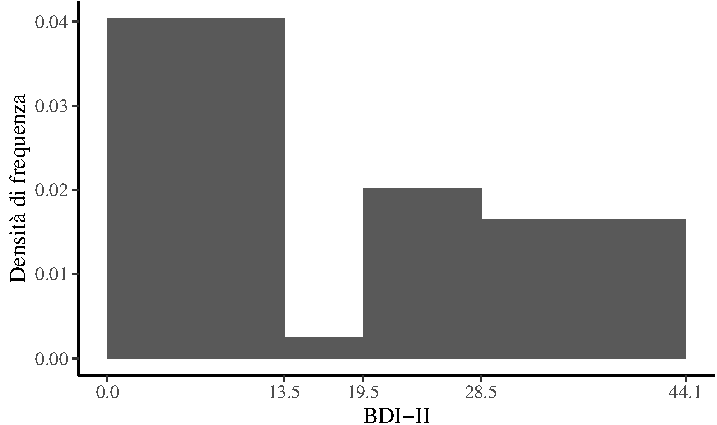
\includegraphics[width=0.8\linewidth]{013_eda_files/figure-latex/hist1zetsche-1} 

}

\caption{Istogramma per i valori BDI-II riportati da Zetsche et al. (2019).}\label{fig:hist1zetsche}
\end{figure}

Con i quattro intervalli individuati dai cut-off del BDI-II otteniamo la
rappresentazione riportata nella figura \ref{fig:hist1zetsche}. Per chiarezza, precisiamo che \texttt{ggplot()} utilizza intervalli aperti a destra.

Nel caso della prima barra dell'istogramma, l'ampiezza dell'intervallo è pari a 13.5 e l'area della barra (ovvero, la frequenza relativa) è uguale a 36/66. Dunque l'altezza della barra è uguale a \((36 / 66) / 13.5 = 0.040\). Lo stesso procedimento si applica per il calcolo dell'altezza degli altri rettangoli.

Anche se nel caso presente è sensato usare ampiezze diverse per gli intervalli delle classi, in generale gli istogrammi si costruiscono utilizzando intervalli riportati sulle ascisse con un'ampiezza uguale. Questo è il caso dell'istogramma della figura \ref{fig:hist2zetsche}.

\begin{Shaded}
\begin{Highlighting}[]
\NormalTok{bysubj }\SpecialCharTok{\%\textgreater{}\%}
  \FunctionTok{ggplot}\NormalTok{(}\FunctionTok{aes}\NormalTok{(}\AttributeTok{x =}\NormalTok{ bdi)) }\SpecialCharTok{+}
  \FunctionTok{geom\_histogram}\NormalTok{(}
    \FunctionTok{aes}\NormalTok{(}\AttributeTok{y =}\NormalTok{ ..density..),}
    \AttributeTok{breaks =} \FunctionTok{seq}\NormalTok{(}\DecValTok{0}\NormalTok{, }\FloatTok{44.1}\NormalTok{, }\AttributeTok{length.out =} \DecValTok{7}\NormalTok{)}
\NormalTok{  ) }\SpecialCharTok{+}
  \FunctionTok{scale\_x\_continuous}\NormalTok{(}
    \AttributeTok{breaks =} \FunctionTok{c}\NormalTok{(}\FloatTok{0.00}\NormalTok{, }\FloatTok{7.35}\NormalTok{, }\FloatTok{14.70}\NormalTok{, }\FloatTok{22.05}\NormalTok{, }
               \FloatTok{29.40}\NormalTok{, }\FloatTok{36.75}\NormalTok{, }\FloatTok{44.10}\NormalTok{)}
\NormalTok{  ) }\SpecialCharTok{+}
  \FunctionTok{labs}\NormalTok{(}
    \AttributeTok{x =} \StringTok{"BDI{-}II"}\NormalTok{,}
    \AttributeTok{y =} \StringTok{"Densità di frequanza"}
\NormalTok{  ) }
\end{Highlighting}
\end{Shaded}

\begin{figure}[h]

{\centering 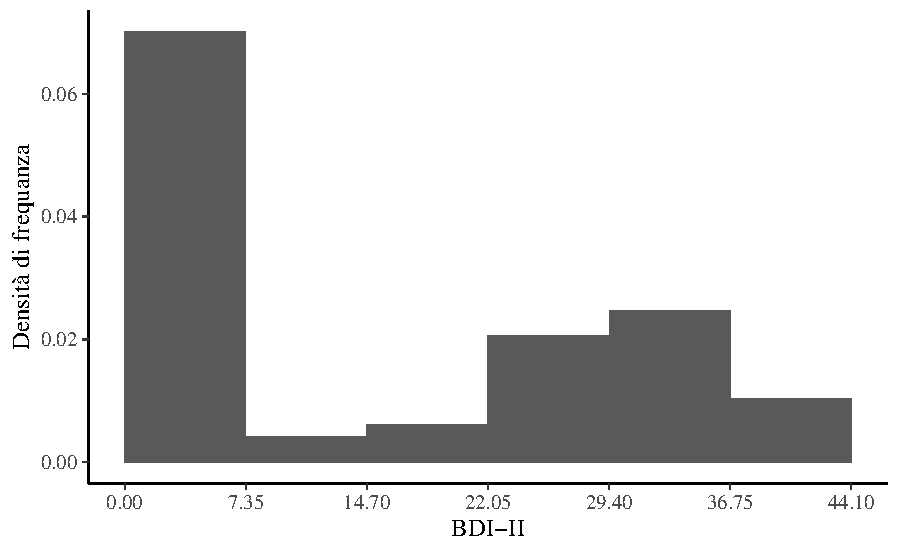
\includegraphics[width=0.8\linewidth]{013_eda_files/figure-latex/hist2zetsche-1} 

}

\caption{Una rappresentazione più comune per l'istogramma dei valori BDI-II nella quale gli intervalli delle classi hanno ampiezze uguali.}\label{fig:hist2zetsche}
\end{figure}

\hypertarget{kernel-density-plot}{%
\section{Kernel density plot}\label{kernel-density-plot}}

Il confronto tra le figure \ref{fig:hist1zetsche} e \ref{fig:hist2zetsche} rende chiaro il limite dell'istogramma: il profilo dell'istogramma è arbitrario, in quanto dipende dal numero e dall'ampiezza delle classi. Questo rende difficile l'interpretazione.

Il problema precedente può essere alleviato utilizzando una
rappresentazione alternativa della distribuzione di frequenza, ovvero la
stima della densità della frequenza dei dati (detta anche stima \emph{kernel
di densità}). Un modo semplice per pensare a tale rappresentazione, che
in inglese va sotto il nome di \emph{kernel density plot} (cioè i grafici basati sulla stima kernel di densità), è quello di immaginare un grande campione di dati, in modo che diventi possibile definire un enorme numero di classi di equivalenza di ampiezza molto piccola, le quali non risultino vuote. In tali circostanze, la funzione di densità empirica non è altro che il profilo \emph{lisciato} dell'istogramma. La stessa idea si applica anche quando il campione è piccolo. In tali circostanze, invece di raccogliere le osservazioni in barre come negli istogrammi, lo stimatore di densità kernel colloca una piccola ``gobba'' (\emph{bump}), determinata da un fattore \(K\) (kernel) e da un parametro \(h\) di smussamento detto ampiezza di banda (\emph{bandwidth}), in corrispondenza di ogni osservazione, quindi somma le gobbe risultanti generando una curva smussata.

L'interpretazione che possiamo attribuire al kernel density plot è simile a quella che viene assegnata agli istogrammi: l'area sottesa al kernel density plot in un certo intervallo rappresenta la proporzione di casi della distribuzione che hanno valori compresi in quell'intervallo.

\begin{example}

Vediamo ora come rappresentare con R sia l'istogramma sia il kernel density plot di una variabile numerica impiegando i valori BDI-II di \textcite{zetschefuture2019}.

\begin{Shaded}
\begin{Highlighting}[]
\NormalTok{bysubj }\SpecialCharTok{\%\textgreater{}\%} 
  \FunctionTok{ggplot}\NormalTok{(}\FunctionTok{aes}\NormalTok{(}\AttributeTok{x =}\NormalTok{ bdi)) }\SpecialCharTok{+}
  \FunctionTok{geom\_histogram}\NormalTok{(}
    \FunctionTok{aes}\NormalTok{(}\AttributeTok{y =}\NormalTok{ ..density..), }
    \AttributeTok{breaks =} \FunctionTok{seq}\NormalTok{(}\DecValTok{0}\NormalTok{, }\FloatTok{44.1}\NormalTok{, }\AttributeTok{length.out =} \DecValTok{7}\NormalTok{)}
\NormalTok{  ) }\SpecialCharTok{+}
  \FunctionTok{geom\_density}\NormalTok{(}
    \FunctionTok{aes}\NormalTok{(}\AttributeTok{x =}\NormalTok{ bdi), }
    \AttributeTok{adjust =} \FloatTok{0.5}\NormalTok{, }
    \AttributeTok{size =} \FloatTok{0.8}\NormalTok{, }
    \CommentTok{\#fill = colors[2],}
    \AttributeTok{alpha =} \FloatTok{0.5}
\NormalTok{  ) }\SpecialCharTok{+}
  \FunctionTok{labs}\NormalTok{(}
    \AttributeTok{x =} \StringTok{"BDI{-}II"}\NormalTok{,}
    \AttributeTok{y =} \StringTok{"Densità di frequenza"}
\NormalTok{  ) }
\end{Highlighting}
\end{Shaded}

\begin{figure}[h]

{\centering 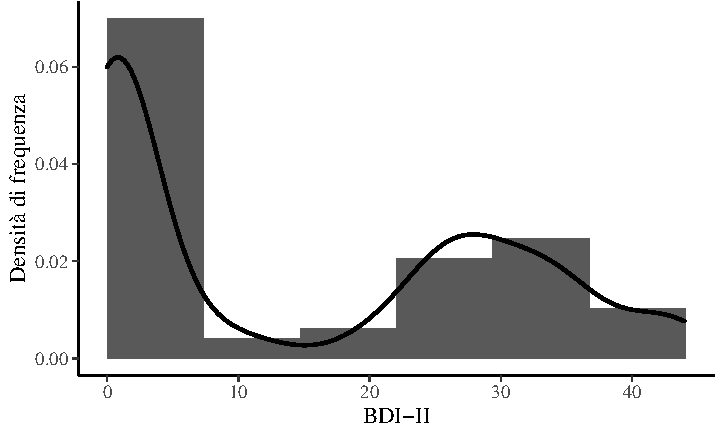
\includegraphics[width=0.8\linewidth]{013_eda_files/figure-latex/zetschehist3-1} 

}

\caption{Kernel density plot e corrispondente istogramma per i valori BDI-II.}\label{fig:zetschehist3}
\end{figure}

\end{example}

\hypertarget{forma-di-una-distribuzione}{%
\section{Forma di una distribuzione}\label{forma-di-una-distribuzione}}

In generale, la forma di una distribuzione descrive come i dati si distribuiscono intorno ai valori centrali. Distinguiamo tra distribuzioni simmetriche e asimmetriche, e tra distribuzioni unimodali o multimodali. Un'illustrazione grafica è fornita nella figura \ref{fig:distrib-shapes}. Nel pannello 1 la distribuzione è unimodale con asimmetria negativa; nel pannello 2 la distribuzione è unimodale con asimmetria positiva; nel pannello 3 la distribuzione è simmetrica e unimodale; nel pannello 4 la distribuzione è bimodale.

\begin{figure}[h]

{\centering 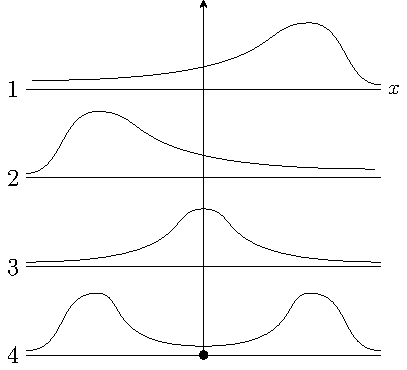
\includegraphics[width=0.8\linewidth]{013_eda_files/figure-latex/distrib-shapes-1} 

}

\caption{1: Asimmetria negativa. 2: Asimmetria positiva. 3: Distribuzione unimodale. 4: Distribuzione bimodale.}\label{fig:distrib-shapes}
\end{figure}

\begin{example}
Il kernel density plot della figura \ref{fig:zetschehist3} indica che la distribuzione dei valori del BDI-II nel campione di \textcite{zetschefuture2019} è bimodale. Ciò indica che le osservazioni della distribuzione si addensano in due cluster ben distinti: un gruppo di osservazioni tende ad avere valori BDI-II bassi, mentre l'altro gruppo tende ad avere BDI-II alti. Questi due cluster di osservazioni corrispondono al gruppo di controllo e al gruppo clinico nel campione di dati esaminato da \textcite{zetschefuture2019}.
\end{example}

\hypertarget{indici-di-posizione}{%
\section{Indici di posizione}\label{indici-di-posizione}}

Nuovamente, se preferite un'introduzione ``soft'' alla nozione di ``tendenza centrale'' di una distribuzione statistica, vi rimando nuovamentew al \href{https://tinystats.github.io/teacups-giraffes-and-statistics/03_mean.html}{link} che ho già suggerito in precedenza.

\hypertarget{quantili}{%
\subsection{Quantili}\label{quantili}}

La descrizione della distribuzione dei valori BDI-II di
\textcite{zetschefuture2019} può essere facilitata dalla determinazione di
alcuni valori caratteristici che sintetizzano le informazioni contenute
nella distribuzione di frequenze. Si dicono \emph{quantili} (o \emph{frattili})
quei valori caratteristici che hanno le seguenti proprietà. I \emph{quartili}
sono quei valori che ripartiscono i dati \(x_i\) in quattro parti
ugualmente numerose (pari ciascuna al 25\% del totale). Il primo
quartile, \(q_1\), lascia alla sua sinistra il 25\% del campione pensato
come una fila ordinata (a destra quindi il 75\%). Il secondo quartile
\(q_2\) lascia a sinistra il 50\% del campione (a destra quindi il 50\%).
Esso viene anche chiamato \emph{mediana}. Il terzo quartile lascia a sinistra
il 75\% del campione (a destra quindi il 25\%). Secondo lo stesso
criterio, si dicono \emph{decili} i quantili di ordine \(p\) multiplo di 0.10 e
\emph{percentili} i quantili di ordine \(p\) multiplo di 0.01.

Come si calcolano i quantili? Consideriamo la definizione di quantile
\emph{non interpolato} di ordine \(p\) \((0 < p < 1)\). Si procede innanzitutto
ordinando i dati in ordine crescente, \(\{x_1, x_2, \dots, x_n\}\). Ci
sono poi due possibilità. Se il valore \(np\) non è intero, sia \(k\)
l'intero tale che \(k < np < k + 1\) -- ovvero, la parte intera di \(np\).
Allora \(q_p = x_{k+1}.\) Se \(np = k\) con \(k\) intero, allora
\(q_p = \frac{1}{2}(x_{k} + x_{k+1}).\) Se vogliamo calcolare il primo
quartile \(q_1\), ad esempio, utilizziamo \(p = 0.25\). Dovendo calcolare
gli altri quantili basta sostituire a \(p\) il valore appropriato{[}\^{}2{]}.

Gli indici di posizione, tra le altre cose, hanno un ruolo importante,
ovvero vengono utilizzati per creare una rappresentazione grafica di una
distribuzione di valori che è molto popolare e può essere usata in
alternativa ad un istogramma (in realtà vedremo poi come possa essere
combinata con un istogramma). Tale rappresentazione va sotto il nome di
box-plot.

\begin{example}
Per fare un esempio, consideriamo i nove soggetti del campione clinico di \textcite{zetschefuture2019} che hanno riportato un unico episodio di depressione maggiore. Per tali soggetti i valori ordinati del BDI-II (per semplicità li chiameremo \(x\)) sono i seguenti: 19, 26, 27, 28, 28, 33, 33, 41, 43.
Per il calcolo del secondo quartile (non interpolato), ovvero per il calcolo della mediana, dobbiamo considerare la quantità \(np = 9 \cdot 0.5 = 4.5\), non intero. Quindi, \(q_1 = x_{4 + 1} = 27\).
Per il calcolo del quantile (non interpolato) di ordine \(p = 2/3\) dobbiamo considerare la quantità \(np = 9 \cdot 2/3 = 6\), intero. Quindi, \(q_{\frac{2}{3}} = \frac{1}{2} (x_{6} + x_{7}) = \frac{1}{2} (33 + 33) = 33\).
\end{example}

\hypertarget{diagramma-a-scatola}{%
\subsection{Diagramma a scatola}\label{diagramma-a-scatola}}

Il \emph{diagramma a scatola} (o box plot) è uno strumento grafico utile al
fine di ottenere informazioni circa la dispersione e l'eventuale
simmetria o asimmetria di una distribuzione. Per costruire un box-plot
si rappresenta sul piano cartesiano un rettangolo (cioè la ``scatola'') di
altezza arbitraria la cui base corrisponde alla dist intanza
interquartile (IQR = \(q_{0.75} - q_{0.25}\)). La linea interna alla
scatola rappresenta la mediana \(q_{0.5}\). Si tracciano poi ai lati della
scatola due segmenti di retta i cui estremi sono detti ``valore
adiacente'' inferiore e superiore. Il valore adiacente inferiore è il
valore più piccolo tra le osservazioni che risulta maggiore o uguale al
primo quartile meno la distanza corrispondente a 1.5 volte la distanza
interquartile.
Il valore adiacente superiore è il valore più grande tra le osservazioni che risulta minore o uguale a \(Q_3+1.5\) IQR. I valori esterni ai valori adiacenti (chiamati \emph{valori anomali}) vengono rappresentati individualmente nel box-plot per meglio evidenziarne la presenza e la posizione.

\begin{figure}[h]

{\centering 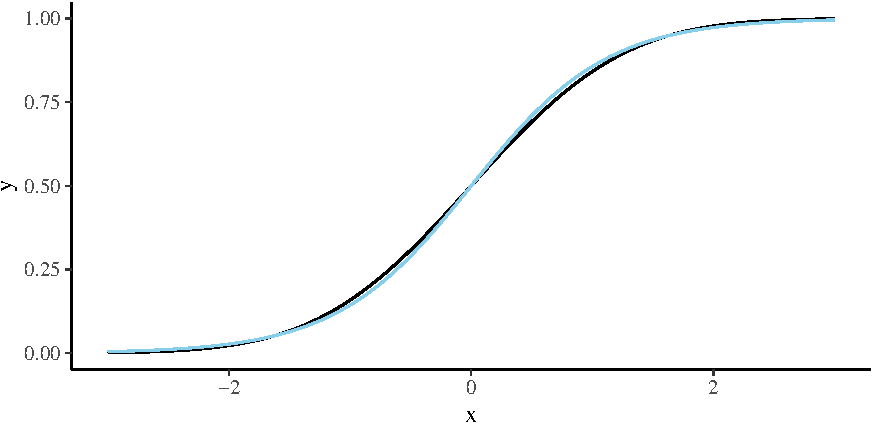
\includegraphics[width=0.8\linewidth]{013_eda_files/figure-latex/unnamed-chunk-9-1} 

}

\caption{Box-plot: $M$ è la mediana, $\bar{x}$ è la media aritmetica e IQR è la distanza interquartile (~$Q_3 - Q_1$~).}\label{fig:unnamed-chunk-9}
\end{figure}

\begin{example}
Consideriamo ora un caso concreto nel quale viene utilizzato un box-plot.
Nel caso dei dati di \textcite{zetschefuture2019} ci chiediamo in che modo si differenziano le distribuzioni del BDI-II tra i due gruppi considerati, ovvero tra il gruppo dei pazienti e il gruppo di controllo. La figura \ref{fig:violin-zetsche} fornisce due rappresentazioni grafiche che possono essere utilizzate per rispondere a questa domanda.

\begin{Shaded}
\begin{Highlighting}[]
\NormalTok{bysubj }\OtherTok{\textless{}{-}}\NormalTok{ df }\SpecialCharTok{\%\textgreater{}\%}
  \FunctionTok{group\_by}\NormalTok{(esm\_id, group) }\SpecialCharTok{\%\textgreater{}\%}
  \FunctionTok{summarise}\NormalTok{(}
    \AttributeTok{bdi =} \FunctionTok{mean}\NormalTok{(bdi),}
    \AttributeTok{nr\_of\_episodes =} \FunctionTok{mean}\NormalTok{(nr\_of\_episodes, }\AttributeTok{na.rm =} \ConstantTok{TRUE}\NormalTok{)}
\NormalTok{  ) }\SpecialCharTok{\%\textgreater{}\%}
  \FunctionTok{na.omit}\NormalTok{() }\SpecialCharTok{\%\textgreater{}\%}
  \FunctionTok{ungroup}\NormalTok{()}

\NormalTok{bysubj}\SpecialCharTok{$}\NormalTok{group }\OtherTok{\textless{}{-}}\NormalTok{ forcats}\SpecialCharTok{::}\FunctionTok{fct\_recode}\NormalTok{(}
\NormalTok{  bysubj}\SpecialCharTok{$}\NormalTok{group,}
  \StringTok{"Controlli}\SpecialCharTok{\textbackslash{}n}\StringTok{ sani"} \OtherTok{=} \StringTok{"ctl"}\NormalTok{,}
  \StringTok{"Depressione}\SpecialCharTok{\textbackslash{}n}\StringTok{ maggiore"} \OtherTok{=} \StringTok{"mdd"}
\NormalTok{)}

\NormalTok{p1 }\OtherTok{\textless{}{-}}\NormalTok{ bysubj }\SpecialCharTok{\%\textgreater{}\%}
  \FunctionTok{ggplot}\NormalTok{(}\FunctionTok{aes}\NormalTok{(}\AttributeTok{x =}\NormalTok{ group, }\AttributeTok{y =}\NormalTok{ bdi)) }\SpecialCharTok{+}
  \FunctionTok{geom\_violin}\NormalTok{(}\AttributeTok{trim =} \ConstantTok{FALSE}\NormalTok{) }\SpecialCharTok{+}
  \FunctionTok{geom\_dotplot}\NormalTok{(}\AttributeTok{binaxis =} \StringTok{"y"}\NormalTok{, }\AttributeTok{stackdir =} \StringTok{"center"}\NormalTok{, }\AttributeTok{dotsize =} \FloatTok{0.7}\NormalTok{) }\SpecialCharTok{+}
  \FunctionTok{labs}\NormalTok{(}
    \AttributeTok{x =} \StringTok{""}\NormalTok{,}
    \AttributeTok{y =} \StringTok{"BDI{-}II"}
\NormalTok{  )}
\NormalTok{p2 }\OtherTok{\textless{}{-}}\NormalTok{ bysubj }\SpecialCharTok{\%\textgreater{}\%}
  \FunctionTok{ggplot}\NormalTok{(}\FunctionTok{aes}\NormalTok{(}\AttributeTok{x =}\NormalTok{ group, }\AttributeTok{y =}\NormalTok{ bdi)) }\SpecialCharTok{+}
  \FunctionTok{geom\_violin}\NormalTok{(}\AttributeTok{trim =} \ConstantTok{FALSE}\NormalTok{) }\SpecialCharTok{+}
  \FunctionTok{geom\_boxplot}\NormalTok{(}\AttributeTok{width =} \FloatTok{0.05}\NormalTok{) }\SpecialCharTok{+}
  \FunctionTok{labs}\NormalTok{(}
    \AttributeTok{x =} \StringTok{""}\NormalTok{,}
    \AttributeTok{y =} \StringTok{"BDI{-}II"}
\NormalTok{  )}
\NormalTok{p1 }\SpecialCharTok{+}\NormalTok{ p2}
\end{Highlighting}
\end{Shaded}

\begin{figure}[h]

{\centering 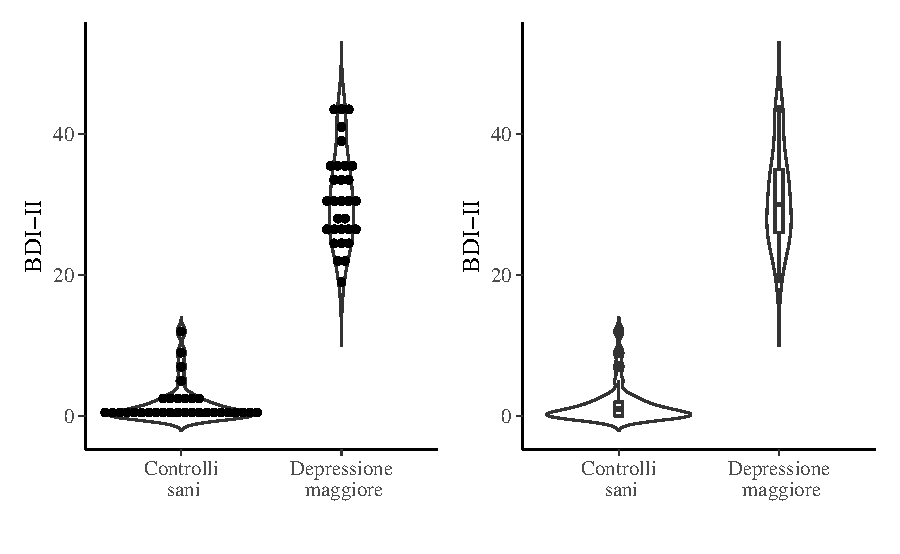
\includegraphics[width=0.8\linewidth]{013_eda_files/figure-latex/violin-zetsche-1} 

}

\caption{Due versioni di un violin plot per i valori BDI-II di ciascuno dei due gruppi di soggetti esaminati da Zetsche et al. (2019).}\label{fig:violin-zetsche}
\end{figure}

Nella figura \ref{fig:violin-zetsche} sinistra sono rappresentati i dati grezzi. La linea curva che circonda (simmetricamente) le osservazioni è l'\emph{istogramma lisciato} (kernel density plot) che abbiamo descritto in precedenza. Nella figura \ref{fig:violin-zetsche} destra sono rappresentanti gli stessi dati: il kernel density plot è lo stesso di prima, ma al suo interno è stato collocato un box-plot. Entrambe le rappresentazioni suggeriscono che la distribuzione dei dati è all'incirca simmetrica nel gruppo clinico. Il gruppo di controllo mostra invece un'asimmetria positiva.
\end{example}

Si noti che i box plot non sono necessariamente la rappresentazione migliore della distribuzione di una variabile. Infatti, richiedono la comprensione di concetti complessi (quali i quantili e la differenza interquantile) che non sono necessari se vogliamo presentare in maniera grafica la distribuzione della variabile e, in generale, non sono compresi da un pubblico di non specialisti. Inoltre, i box plot nascondono informazioni che di solito sono cruciali da vedere. È dunque preferibile presentare direttamente i dati.

Qui di seguito viene presentato un cosiddetto ``sina plot''. In tale rappresentazione grafica vengono mostrate le singole osservazioni divise in classi. Ai punti viene aggiunto un jitter, così da evitare sovrapposizioni. L'ampiezza del jitter lungo l'asse \(x\) è determinata dalla distribuzione della densità dei dati all'interno di ciascuna classe; quindi il grafico mostra lo stesso contorno di un \emph{violin plot}, ma trasmette informazioni sia sul numero di punti dati, sia sulla distribuzione della densità, sui valori anomali e sulla distribuzione dei dati in un formato molto semplice, comprensibile e sintetico. Per i dati dell'esempio in discussione, otteniamo la rappresentazione della figura \ref{fig:sina-zetsche}, a cui è stata aggiunta la mediana di ciascun gruppo.

\begin{Shaded}
\begin{Highlighting}[]
\NormalTok{zetsche\_summary }\OtherTok{\textless{}{-}}\NormalTok{ bysubj }\SpecialCharTok{\%\textgreater{}\%}
  \FunctionTok{group\_by}\NormalTok{(group) }\SpecialCharTok{\%\textgreater{}\%}
  \FunctionTok{summarize}\NormalTok{(}
    \AttributeTok{bdi\_mean =} \FunctionTok{mean}\NormalTok{(bdi),}
    \AttributeTok{bdi\_sd =} \FunctionTok{sd}\NormalTok{(bdi),}
    \AttributeTok{bdi\_median =} \FunctionTok{median}\NormalTok{(bdi)}
\NormalTok{  ) }\SpecialCharTok{\%\textgreater{}\%} 
  \FunctionTok{ungroup}\NormalTok{()}

\NormalTok{bysubj }\SpecialCharTok{\%\textgreater{}\%}
  \FunctionTok{ggplot}\NormalTok{(}
    \FunctionTok{aes}\NormalTok{(}\AttributeTok{x =}\NormalTok{ group, }\AttributeTok{y =}\NormalTok{ bdi, }\AttributeTok{color =}\NormalTok{ group)}
\NormalTok{  ) }\SpecialCharTok{+}
\NormalTok{  ggforce}\SpecialCharTok{::}\FunctionTok{geom\_sina}\NormalTok{(}\FunctionTok{aes}\NormalTok{(}\AttributeTok{color =}\NormalTok{ group, }\AttributeTok{size =} \DecValTok{3}\NormalTok{, }\AttributeTok{alpha =}\NormalTok{ .}\DecValTok{5}\NormalTok{)) }\SpecialCharTok{+}
  \FunctionTok{geom\_errorbar}\NormalTok{(}
    \FunctionTok{aes}\NormalTok{(}\AttributeTok{y =}\NormalTok{ bdi\_median, }\AttributeTok{ymin =}\NormalTok{ bdi\_median, }\AttributeTok{ymax =}\NormalTok{ bdi\_median),}
    \AttributeTok{data =}\NormalTok{ zetsche\_summary, }\AttributeTok{width =} \FloatTok{0.3}\NormalTok{, }\AttributeTok{size =} \DecValTok{3}
\NormalTok{  ) }\SpecialCharTok{+}
  \FunctionTok{scale\_color\_okabe\_ito}\NormalTok{(}\AttributeTok{name =} \StringTok{"group"}\NormalTok{, }\AttributeTok{alpha =}\NormalTok{ .}\DecValTok{9}\NormalTok{) }\SpecialCharTok{+}
  \FunctionTok{labs}\NormalTok{(}
    \AttributeTok{x =} \StringTok{""}\NormalTok{,}
    \AttributeTok{y =} \StringTok{"BDI{-}II"}\NormalTok{,}
    \AttributeTok{color =} \StringTok{"Gruppo"}
\NormalTok{  ) }\SpecialCharTok{+}
  \FunctionTok{theme}\NormalTok{(}\AttributeTok{legend.position =} \StringTok{"none"}\NormalTok{)}
\end{Highlighting}
\end{Shaded}

\begin{figure}[h]

{\centering 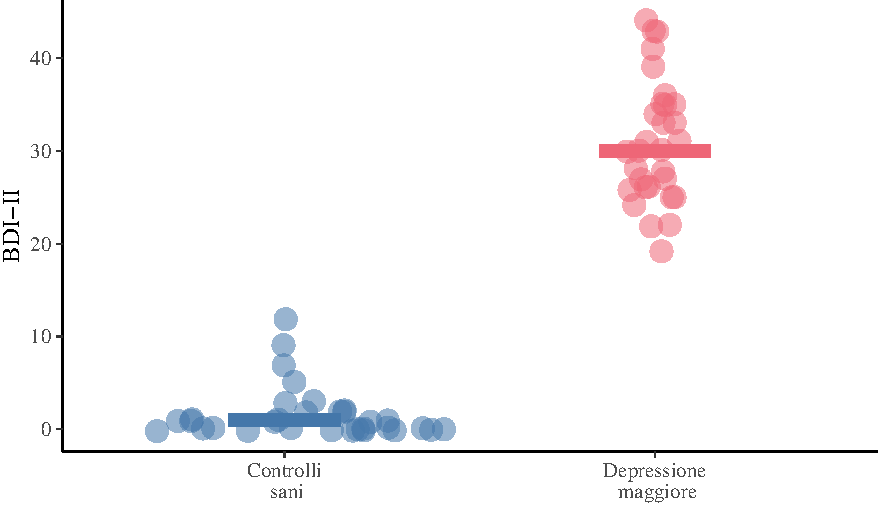
\includegraphics[width=0.8\linewidth]{013_eda_files/figure-latex/sina-zetsche-1} 

}

\caption{Sina plot per i valori BDI-II di ciascuno dei due gruppi di soggetti esaminati da Zetsche et al. (2019) con l'indicazione della mediana per ciascun gruppo.}\label{fig:sina-zetsche}
\end{figure}

\hypertarget{leccellenza-grafica}{%
\subsection{L'eccellenza grafica}\label{leccellenza-grafica}}

Non c'è un modo ``corretto'' per rappresentare in forma grafica un insieme
di dati. Ciascuno dei grafici che abbiamo discusso in precedenza ha i suoi pregi e i suoi difetti. Un ricercatore che ha molto influenzato il modo in cui
viene realizzata la visualizzazione dei dati scientifici è Edward Tufte,
soprannominato dal New York Times il ``Leonardo da Vinci dei dati.''
Secondo Tufte, ``l'eccellenza nella grafica consiste nel comunicare idee
complesse in modo chiaro, preciso ed efficiente''. Nella visualizzazione
delle informazioni, l'``eccellenza grafica'' ha l'obiettivo di comunicare
al lettore il maggior numero di idee nella maniera più diretta e semplice possibile. Secondo \textcite{tufte_visual_display}, le rappresentazioni grafiche dovrebbero:

\begin{enumerate}
\def\labelenumi{\arabic{enumi}.}
\tightlist
\item
  mostrare i dati;
\item
  indurre l'osservatore a riflettere sulla sostanza piuttosto che
  sulla progettazione grafica, o qualcos'altro;
\item
  evitare di distorcere quanto i dati stanno comunicando (``integrità
  grafica'');
\item
  presentare molte informazioni in forma succinta;
\item
  rivelare la coerenza tra le molte dimensioni dei dati;
\item
  incoraggiare l'osservatore a confrontare differenti sottoinsiemi di dati;
\item
  rivelare i dati a diversi livelli di dettaglio, da una visione ampia
  alla struttura di base;
\item
  servire ad uno scopo preciso (descrizione, esplorazione, o la
  risposta a qualche domanda);
\item
  essere fortemente integrate con le descrizioni statistiche e verbali
  dei dati fornite nel testo.
\end{enumerate}

In base a questi principi, figura \ref{fig:sina-zetsche} sembra fornire la
rappresentazione migliore dei dati di \textcite{zetschefuture2019}. Il seguente \href{https://www.biostat.wisc.edu/~kbroman/presentations/graphs2018.pdf}{link} fornisce diverse interessanti illustrazioni dei principi elencati sopra.

\hypertarget{indici-di-tendenza-centrale}{%
\section{Indici di tendenza centrale}\label{indici-di-tendenza-centrale}}

L'analisi grafica, esaminata in precedenza, costituisce la base di
partenza di qualsivoglia analisi quantitativa dei dati. Tramite
l'analisi grafica possiamo capire alcune caratteristiche importanti di
una distribuzione: per esempio, se è simmetrica o asimmetrica; oppure se
è unimodale o multimodale. Successivamente, possiamo calcolare degli
indici numerici che descrivono in modo sintetico le caratteristiche di
base dei dati esaminati. Tra le misure di tendenza centrale, ovvero tra
gli indici che forniscono un'idea dei valori attorno ai quali sono
prevalentemente concentrati i dati di un campione, quella più
comunemente usata è la media.

\hypertarget{media}{%
\subsection{Media}\label{media}}

Tutti conosciamo la media aritmetica di \(\{x_1, x_2, \dots, x_n\}\),
ovvero il numero reale \(\bar{x}\) definito da
\begin{equation}
\bar{x}=\frac{1}{n}\sum_{i=1}^n x_i.
\label{eq:mean}
\end{equation}
Nell'eq. \eqref{eq:mean} abbiamo usato la notazione delle sommatorie
per descrivere una somma di valori. Questa notazione è molto usata in
statistica e viene descritta in Appendice.

La media gode della seguente importante proprietà: la somma degli scarti
tra ciascuna modalità \(x_i\) e la media aritmetica \(\bar{x}\) è nulla,
cioè
\[
\sum_{i=1}^n (x_i - \bar{x}) = 0.\notag
\label{eq:diffmeansumzero}\] Infatti, \[\begin{aligned}
\sum_{i=1}^n (x_i - \bar{x}) &= \sum_i x_i - \sum_i \bar{x}\notag\\
&= \sum_i x_i - n \bar{x}\notag\\
&= \sum_i x_i - \sum_i x_i = 0.\notag\end{aligned}
\]
Ciò ci consente di pensare alla media come al baricentro della distribuzione.

Un'altra proprietà della media è la seguente. La somma dei quadrati
degli scarti tra ciascuna modalità \(x_i\) e una costante arbitraria
\(a \in \Re\), cioè \[\varphi(a) = \sum_{i=1}^n (x_i - a)^2,\notag\] è
minima per \(a = \bar{x}\).

Il concetto statistico di media ha suscitato molte battute. Per esempio,
il fatto che, in media, ciascuno di noi ha un numero di gambe circa pari
a 1.9999999. Oppure, il fatto che, in media, ciascuno di noi ha un
testicolo. Ma la media ha altri problemi, oltre al fatto di ispirare
battute simili alle precedenti. In particolare, dobbiamo notare che la
media non è sempre l'indice che meglio rappresenta la tendenza centrale
di una distribuzione. In particolare, ciò non accade quando la
distribuzione è asimmetrica, o in presenza di valori anomali (\emph{outlier})
-- si veda il pannello di destra della figura \ref{fig:violin-zetsche}. In tali circostanze, la tendenza centrale della distribuzione è meglio rappresentata dalla mediana o dalla media spuntata.

\begin{example}

Calcoliamo la media dei valori BDI-II per i due gruppi di soggetti di \textcite{zetschefuture2019}.

\begin{Shaded}
\begin{Highlighting}[]
\NormalTok{bysubj }\SpecialCharTok{\%\textgreater{}\%} 
  \FunctionTok{group\_by}\NormalTok{(group) }\SpecialCharTok{\%\textgreater{}\%} 
  \FunctionTok{summarise}\NormalTok{(}
    \AttributeTok{avg\_bdi =} \FunctionTok{mean}\NormalTok{(bdi)}
\NormalTok{  ) }
\CommentTok{\#\textgreater{} \# A tibble: 2 x 2}
\CommentTok{\#\textgreater{}   group                    avg\_bdi}
\CommentTok{\#\textgreater{}   \textless{}fct\textgreater{}                      \textless{}dbl\textgreater{}}
\CommentTok{\#\textgreater{} 1 "Controlli\textbackslash{}n sani"          1.69}
\CommentTok{\#\textgreater{} 2 "Depressione\textbackslash{}n maggiore"   30.9}
\end{Highlighting}
\end{Shaded}

\end{example}

\hypertarget{media-spuntata}{%
\subsection{Media spuntata}\label{media-spuntata}}

La \emph{media spuntata} \(\bar{x}_t\) (\emph{trimmed mean}) non è altro che la
media dei dati calcolata considerando solo il 90\% (o altra percentuale)
dei dati centrali. Per calcolare \(\bar{x}_t\) si ordinando i dati secondo
una sequenza crescente, \(x_1 \leq x_2 \leq x_3 \leq \dots \leq x_n\), per
poi eliminare il primo 5\% e l'ultimo 5\% dei dati della serie così
ordinata. La media spuntata è data dalla media aritmetica dei dati rimanenti.

\begin{example}

Calcoliamo la media spuntata dei valori BDI-II per i due gruppi di soggetti di \textcite{zetschefuture2019} escludendo il 10\% dei valori più estremi in ciascun gruppo.

\begin{Shaded}
\begin{Highlighting}[]
\NormalTok{bysubj }\SpecialCharTok{\%\textgreater{}\%} 
  \FunctionTok{group\_by}\NormalTok{(group) }\SpecialCharTok{\%\textgreater{}\%} 
  \FunctionTok{summarise}\NormalTok{(}
    \AttributeTok{avg\_trim\_bdi =} \FunctionTok{mean}\NormalTok{(bdi, }\AttributeTok{trim =} \FloatTok{0.1}\NormalTok{)}
\NormalTok{  ) }
\CommentTok{\#\textgreater{} \# A tibble: 2 x 2}
\CommentTok{\#\textgreater{}   group                    avg\_trim\_bdi}
\CommentTok{\#\textgreater{}   \textless{}fct\textgreater{}                           \textless{}dbl\textgreater{}}
\CommentTok{\#\textgreater{} 1 "Controlli\textbackslash{}n sani"                1  }
\CommentTok{\#\textgreater{} 2 "Depressione\textbackslash{}n maggiore"         30.6}
\end{Highlighting}
\end{Shaded}

\end{example}

\hypertarget{moda-e-mediana}{%
\subsection{Moda e mediana}\label{moda-e-mediana}}

In precedenza abbiamo già incontrato altri due popolari indici di
tendenza centrale: la \emph{moda} (\emph{Mo}), ovvero il valore centrale della
classe con la frequenza massima (può succedere che una distribuzione
abbia più mode; in tal caso si dice \emph{multimodale} e questo operatore
perde il suo significato di indice di tendenza centrale) e la \emph{mediana}
\(\tilde{x}\).

\begin{example}

Calcoliamo i quantili di ordine 0.25, 0.5 e 0.75 dei valori BDI-II per i due gruppi di soggetti di \textcite{zetschefuture2019}.

\begin{Shaded}
\begin{Highlighting}[]
\NormalTok{bysubj }\SpecialCharTok{\%\textgreater{}\%} 
  \FunctionTok{group\_by}\NormalTok{(group) }\SpecialCharTok{\%\textgreater{}\%} 
  \FunctionTok{summarise}\NormalTok{(}
    \AttributeTok{q25 =} \FunctionTok{quantile}\NormalTok{(bdi, }\AttributeTok{probs =} \FloatTok{0.25}\NormalTok{),}
    \AttributeTok{q50 =} \FunctionTok{quantile}\NormalTok{(bdi, }\AttributeTok{probs =} \FloatTok{0.50}\NormalTok{),}
    \AttributeTok{q75 =} \FunctionTok{quantile}\NormalTok{(bdi, }\AttributeTok{probs =} \FloatTok{0.75}\NormalTok{)}
\NormalTok{  ) }
\CommentTok{\#\textgreater{} \# A tibble: 2 x 4}
\CommentTok{\#\textgreater{}   group                      q25   q50   q75}
\CommentTok{\#\textgreater{}   \textless{}fct\textgreater{}                    \textless{}dbl\textgreater{} \textless{}dbl\textgreater{} \textless{}dbl\textgreater{}}
\CommentTok{\#\textgreater{} 1 "Controlli\textbackslash{}n sani"           0     1     2}
\CommentTok{\#\textgreater{} 2 "Depressione\textbackslash{}n maggiore"    26    30    35}
\end{Highlighting}
\end{Shaded}

\end{example}

Si noti che solitamente i software restituiscono un valore \textbf{interpolato} del \(p\)-esimo quantile \(q_p\) \((0 < p < 1)\), il quale viene calcolato mediante specifiche procedure. Il risultato fornito dai software, dunque, non sarà identico a quello trovato utilizzando la definizione non interpolata di quantile che abbiamo presentato qui. Se, per qualche ragione, vogliamo conoscere l'algoritmo usato per la determinazione dei quantili interpolati, dobbiamo leggere la documentazione del software.

\hypertarget{indici-di-dispersione}{%
\section{Indici di dispersione}\label{indici-di-dispersione}}

Le medie e gli indici di posizione descritti in precedenza forniscono
delle sintesi dei dati che mettono in evidenza la tendenza centrale
delle osservazioni. Tali indici, tuttavia, non considerano un aspetto
importante della distribuzione dei dati, ovvero la variabilità dei
valori numerici della variabile statistica. È dunque necessario
sintetizzare la distribuzione di una variabile statistica oltre che con
le misure di posizione anche tramite l'utilizzo di indicatori che
valutino la dispersione delle unità statistice.

Anche in questo caso, un'introduzione ``soft'' è fornita nel \href{https://tinystats.github.io/teacups-giraffes-and-statistics/04_variance.html}{link}.

\hypertarget{indici-basati-sullordinamento-dei-dati}{%
\subsection{Indici basati sull'ordinamento dei dati}\label{indici-basati-sullordinamento-dei-dati}}

È possibile calcolare degli indici di variabilità basati
sull'ordinamento dei dati. L'indice più ovvio è l'intervallo di
variazione, ovvero la distanza tra il valore massimo e il valore minimo
di una distribuzione di modalità, mentre in precedenza abbiamo già
incontrato la differenza interquartile. Questi due indici, però, hanno
il limite di essere calcolati sulla base di due soli valori della
distribuzione (\(x_{\text{max}}\) e \(x_{\text{mini}}\), oppure \(x_{0.25}\) e
\(x_{0.75}\)). Pertanto non utilizzano tutte le informazioni che sono
disponibili. Inoltre, l'intervallo di variazione ha il limite di essere
pesantemente influenzato dalla presenza di valori anomali.

\hypertarget{varianza}{%
\subsection{Varianza}\label{varianza}}

Dati i limiti delle statistiche precedenti è più comune misurare la
variabilità di una variabile statistica come la dispersione dei dati
attorno ad un indice di tendenza centrale. Infatti, la misura di variabilità di gran lunga più usata per valutare la variabilità di una variabile statistica è senza dubbio la varianza. La varianza
\begin{equation}
s^2 = \frac{1}{n} \sum_{i=1}^n (x_i - \bar{x})^2
\label{eq:var-descr}
\end{equation}
è la media dei quadrati degli scarti \(x_i - \bar{x}\) tra ogni valore e la media della distribuzione.
La varianza è una misura di dispersione più complessa di quelle esaminate in precedenza. È appropriata solo nel caso di distribuzioni simmetriche e, anch'essa, è fortemente influenzata dai valori anomali. Inoltre, è espressa in un'unità di misura che è il quadrato dell'unità di misura dei dati originari e quindi ad essa non può essere assegnata un'interpretazione intuitiva.

\begin{example}

Calcoliamo la varianza dei punteggi BDI-II nei due gruppi di soggetti di \textcite{zetschefuture2019}.

\begin{Shaded}
\begin{Highlighting}[]
\NormalTok{bysubj }\SpecialCharTok{\%\textgreater{}\%} 
  \FunctionTok{group\_by}\NormalTok{(group) }\SpecialCharTok{\%\textgreater{}\%} 
  \FunctionTok{summarise}\NormalTok{(}
    \AttributeTok{variance =} \FunctionTok{var}\NormalTok{(bdi)}
\NormalTok{  ) }
\CommentTok{\#\textgreater{} \# A tibble: 2 x 2}
\CommentTok{\#\textgreater{}   group                    variance}
\CommentTok{\#\textgreater{}   \textless{}fct\textgreater{}                       \textless{}dbl\textgreater{}}
\CommentTok{\#\textgreater{} 1 "Controlli\textbackslash{}n sani"           8.03}
\CommentTok{\#\textgreater{} 2 "Depressione\textbackslash{}n maggiore"    43.7}
\end{Highlighting}
\end{Shaded}

\end{example}

\hypertarget{deviazione-standard}{%
\subsection{Deviazione standard}\label{deviazione-standard}}

Per le ragioni espresse sopra, la misura più usata della dispersione di una distribuzione di dati è la \emph{deviazione standard}, ovvero la radice quadrata della varianza. A differenza della varianza, dunque, la deviazione standard è espressa nella stessa unità di misura dei dati. Come nel caso della varianza, anche la deviazione standard \(s\) dovrebbe essere usata soltanto quando la media è adeguata per misurare il centro della distribuzione, ovvero, nel caso di distribuzioni simmetriche. Come nel caso della media \(\bar{x}\), anche la deviazione standard è fortemente influenzata dai dati anomali (\emph{outlier}), ovvero dalla presenza di uno o di pochi dati che sono molto più distanti dalla media rispetto agli altri valori della distribuzione. Quando tutte le osservazioni sono uguali, \(s=0\), altrimenti \(s > 0\).

Alla deviazione standard può essere assegnata una semplice interpretazione: la deviazione standard è \textbf{simile} (ma non identica) allo scostamento medio semplice dalla media. La deviazione standard ci dice, dunque, quanto sono distanti, in media, le singole osservazioni dal centro della distribuzione.

\begin{example}

Calcoliamo la deviazione standard per il BDI-II dei due gruppi di soggetti di \textcite{zetschefuture2019}.

\begin{Shaded}
\begin{Highlighting}[]
\NormalTok{bysubj }\SpecialCharTok{\%\textgreater{}\%} 
  \FunctionTok{group\_by}\NormalTok{(group) }\SpecialCharTok{\%\textgreater{}\%} 
  \FunctionTok{summarise}\NormalTok{(}
    \AttributeTok{stdev =} \FunctionTok{sd}\NormalTok{(bdi)}
\NormalTok{  ) }
\CommentTok{\#\textgreater{} \# A tibble: 2 x 2}
\CommentTok{\#\textgreater{}   group                    stdev}
\CommentTok{\#\textgreater{}   \textless{}fct\textgreater{}                    \textless{}dbl\textgreater{}}
\CommentTok{\#\textgreater{} 1 "Controlli\textbackslash{}n sani"        2.83}
\CommentTok{\#\textgreater{} 2 "Depressione\textbackslash{}n maggiore"  6.61}
\end{Highlighting}
\end{Shaded}

\end{example}

\hypertarget{deviazione-mediana-assoluta}{%
\subsection{Deviazione mediana assoluta}\label{deviazione-mediana-assoluta}}

Una misura robusta della dispersione statistica di un campione è la deviazione mediana assoluta (Median Absolute Deviation, MAD) definita come la mediana del valore assoluto delle deviazioni dei dati dalla mediana, ovvero:
\[
{\displaystyle \operatorname {MAD} =\operatorname {median} \left(\ \left|X_{i}-\operatorname {median} (X)\right|\ \right)}
\]
Nel caso di una distribuzione dei dati unimodale simmetrica di forma campanulare (ovvero, normale) si ha che
\[
{\displaystyle \text{deviazione standard} \approx 1.4826\ \operatorname {MAD} .\,}
\]
Pertanto, solitamente i software restituiscono il valore MAD moltiplicato per una tale costante.

\begin{example}

Calcoliamo il valore MAD per il BDI-II dei due gruppi di soggetti di \textcite{zetschefuture2019}.

\begin{Shaded}
\begin{Highlighting}[]
\FloatTok{1.4826} \SpecialCharTok{*} \FunctionTok{median}\NormalTok{(}\FunctionTok{abs}\NormalTok{(bysubj}\SpecialCharTok{$}\NormalTok{bdi }\SpecialCharTok{{-}} \FunctionTok{median}\NormalTok{(bysubj}\SpecialCharTok{$}\NormalTok{bdi)))}
\CommentTok{\#\textgreater{} [1] 15.6}
\end{Highlighting}
\end{Shaded}

Oppure, per i due gruppi:

\begin{Shaded}
\begin{Highlighting}[]
\NormalTok{bysubj }\SpecialCharTok{\%\textgreater{}\%} 
  \FunctionTok{group\_by}\NormalTok{(group) }\SpecialCharTok{\%\textgreater{}\%} 
  \FunctionTok{summarise}\NormalTok{(}
    \AttributeTok{MAD =} \FunctionTok{mad}\NormalTok{(bdi)}
\NormalTok{  ) }
\CommentTok{\#\textgreater{} \# A tibble: 2 x 2}
\CommentTok{\#\textgreater{}   group                      MAD}
\CommentTok{\#\textgreater{}   \textless{}fct\textgreater{}                    \textless{}dbl\textgreater{}}
\CommentTok{\#\textgreater{} 1 "Controlli\textbackslash{}n sani"        1.48}
\CommentTok{\#\textgreater{} 2 "Depressione\textbackslash{}n maggiore"  6.67}
\end{Highlighting}
\end{Shaded}

\end{example}

\hypertarget{indici-di-variabilituxe0-relativi}{%
\subsection{Indici di variabilità relativi}\label{indici-di-variabilituxe0-relativi}}

A volte può essere interessante effettuare un confronto fra due misure
di variabilità di grandezze incommensurabili, ovvero di caratteri
rilevati mediante differenti unità di misura. In questi casi, le misure
di variabilità precedentemente descritte si rivelano inadeguate in
quanto dipendono dall'unità di misura adottata. Diventa dunque
necessario ricorrere a particolari numeri adimensionali detti indici
relativi di variabilità. Il più importante di tali indici è il
coefficiente di variazione, ovvero il numero puro
\[C_v = \frac{\sigma}{\bar{x}}\] ottenuto dal rapporto tra la deviazione
standard e la media dei dati. Un altro indice relativo di variabilità è
la differenza interquartile rapportata al primo quartile oppure al terzo
quartile oppure alla mediana, cioè:
\[\frac{x_{0.75} - x_{0.25}}{x_{0.25}}, \qquad \frac{x_{0.75} - x_{0.25}}{x_{0.75}}, \qquad \frac{x_{0.75} - x_{0.25}}{x_{0.50}}.\notag\]

\hypertarget{le-relazioni-tra-variabili}{%
\section{Le relazioni tra variabili}\label{le-relazioni-tra-variabili}}

\textcite{zetschefuture2019} hanno misurato il livello di depressione dei
soggetti del loro esperimento utilizzando due scale psicometriche: il
Beck Depression Inventory II (BDI-II) e la Center for Epidemiologic
Studies Depression Scale (CES-D). Il BDI-II è uno strumento self-report
che valutare la presenza e l'intensità di sintomi depressivi in pazienti
adulti e adolescenti di almeno 13 anni di età con diagnosi psichiatrica
mentre la CES-D è una scala self-report progettata per misurare i
sintomi depressivi che sono stati vissuti nella settimana precedente
nella popolazione generale, specialmente quella degli
adolescenti/giovani adulti. Una domanda ovvia che ci può venire in
mente è: quanto sono simili le misure ottenute mediante queste due
scale?

È chiaro che i numeri prodotti dalle scale BDI-II e CES-D non possono
essere identici, e questo per due motivi: (1) la presenza degli errori
di misurazione e (2) l'unità di misura delle due variabili. L'errore di
misurazione corrompe sempre, almeno in parte, qualunque operazione di
misurazione. E questo è vero specialmente in psicologia dove
l'\emph{attendibilità} degli strumenti di misurazione è minore che in altre
discipline (quali la fisica, ad esempio). Il secondo motivo per cui i
valori delle scale BDI-II e CES-D non possono essere uguali è che
l'unità di misura delle due scale è arbitraria. Infatti, qual è l'unità
di misura della depressione? Chi può dirlo! Ma, al di là delle
differenze derivanti dall'errore di misurazione e dalla differente unità
di misura, ci aspettiamo che, se le due scale misurano entrambe lo
stesso costrutto, allora i valori prodotti dalle due scale dovranno
essere tra loro \emph{linearmente associati}. Per capire cosa si intende con
``associazione lineare'' iniziamo a guardare i dati. Per fare questo
utilizziamo una rappresentazione grafica che va sotto il nome di
diagramma a dispersione.

\hypertarget{diagramma-a-dispersione}{%
\subsection{Diagramma a dispersione}\label{diagramma-a-dispersione}}

Il diagramma di dispersione è la rappresentazione grafica delle coppie di punti individuati da due variabili \(X\) e \(Y\).

Il diagramma di dispersione per le variabili BDI-II e CES-D si ottiene ponendo, ad esempio, i valori BDI-II sull'asse delle ascisse e quelli del CES-D sull'asse delle ordinate. In tale grafico, fornito dalla figura~\ref{fig:zetsche-scatter}, cascun punto corrisponde ad un individuo del quale, nel caso presente, conosciamo il livello di depressione misurato dalle due scale psicometriche.

\begin{Shaded}
\begin{Highlighting}[]
\NormalTok{bysubj }\OtherTok{\textless{}{-}}\NormalTok{ df }\SpecialCharTok{\%\textgreater{}\%}
  \FunctionTok{group\_by}\NormalTok{(esm\_id, group) }\SpecialCharTok{\%\textgreater{}\%}
  \FunctionTok{summarise}\NormalTok{(}
    \AttributeTok{bdi =} \FunctionTok{mean}\NormalTok{(bdi),}
    \AttributeTok{cesd =} \FunctionTok{mean}\NormalTok{(cesd\_sum)}
\NormalTok{  ) }\SpecialCharTok{\%\textgreater{}\%}
  \FunctionTok{na.omit}\NormalTok{() }\SpecialCharTok{\%\textgreater{}\%}
  \FunctionTok{ungroup}\NormalTok{()}
\end{Highlighting}
\end{Shaded}

\begin{Shaded}
\begin{Highlighting}[]

\NormalTok{m\_cesd }\OtherTok{\textless{}{-}}\NormalTok{ bysubj }\SpecialCharTok{\%\textgreater{}\%} 
\NormalTok{  dplyr}\SpecialCharTok{::}\FunctionTok{pull}\NormalTok{(cesd) }\SpecialCharTok{\%\textgreater{}\%} 
  \FunctionTok{mean}\NormalTok{()}

\NormalTok{m\_bdi }\OtherTok{\textless{}{-}}\NormalTok{ bysubj }\SpecialCharTok{\%\textgreater{}\%} 
\NormalTok{  dplyr}\SpecialCharTok{::}\FunctionTok{pull}\NormalTok{(bdi) }\SpecialCharTok{\%\textgreater{}\%} 
  \FunctionTok{mean}\NormalTok{()}

\NormalTok{FONT\_SIZE }\OtherTok{\textless{}{-}} \DecValTok{9}

\NormalTok{bysubj }\SpecialCharTok{\%\textgreater{}\%}
  \FunctionTok{ggplot}\NormalTok{(}
    \FunctionTok{aes}\NormalTok{(}\AttributeTok{x =}\NormalTok{ bdi, }\AttributeTok{y =}\NormalTok{ cesd, }\AttributeTok{color =}\NormalTok{ group)}
\NormalTok{  ) }\SpecialCharTok{+}
  \FunctionTok{geom\_point}\NormalTok{(}\AttributeTok{size =} \DecValTok{3}\NormalTok{, }\AttributeTok{alpha =}\NormalTok{ .}\DecValTok{5}\NormalTok{) }\SpecialCharTok{+}
  \FunctionTok{scale\_color\_okabe\_ito}\NormalTok{(}\AttributeTok{name =} \StringTok{"group"}\NormalTok{, }\AttributeTok{alpha =}\NormalTok{ .}\DecValTok{9}\NormalTok{) }\SpecialCharTok{+}
  \FunctionTok{geom\_hline}\NormalTok{(}\AttributeTok{yintercept =}\NormalTok{ m\_cesd, }\AttributeTok{linetype =} \StringTok{"dashed"}\NormalTok{, }\AttributeTok{color =} \StringTok{"gray"}\NormalTok{) }\SpecialCharTok{+}
  \FunctionTok{geom\_vline}\NormalTok{(}\AttributeTok{xintercept =}\NormalTok{ m\_bdi, }\AttributeTok{linetype =} \StringTok{"dashed"}\NormalTok{, }\AttributeTok{color =} \StringTok{"gray"}\NormalTok{) }\SpecialCharTok{+}
  \FunctionTok{geom\_text}\NormalTok{(}\AttributeTok{x =} \SpecialCharTok{{-}}\DecValTok{1}\NormalTok{, }\AttributeTok{y =} \DecValTok{16}\NormalTok{, }\AttributeTok{label =} \StringTok{"I"}\NormalTok{, }\AttributeTok{color =} \StringTok{"gray"}\NormalTok{, }\AttributeTok{size =}\NormalTok{ FONT\_SIZE) }\SpecialCharTok{+}
  \FunctionTok{geom\_text}\NormalTok{(}\AttributeTok{x =} \DecValTok{0}\NormalTok{, }\AttributeTok{y =} \DecValTok{46}\NormalTok{, }\AttributeTok{label =} \StringTok{"IV"}\NormalTok{, }\AttributeTok{color =} \StringTok{"gray"}\NormalTok{, }\AttributeTok{size =}\NormalTok{ FONT\_SIZE) }\SpecialCharTok{+}
  \FunctionTok{geom\_text}\NormalTok{(}\AttributeTok{x =} \DecValTok{18}\NormalTok{, }\AttributeTok{y =} \DecValTok{46}\NormalTok{, }\AttributeTok{label =} \StringTok{"III"}\NormalTok{, }\AttributeTok{color =} \StringTok{"gray"}\NormalTok{, }\AttributeTok{size =}\NormalTok{ FONT\_SIZE) }\SpecialCharTok{+}
  \FunctionTok{geom\_text}\NormalTok{(}\AttributeTok{x =} \DecValTok{18}\NormalTok{, }\AttributeTok{y =} \DecValTok{16}\NormalTok{, }\AttributeTok{label =} \StringTok{"II"}\NormalTok{, }\AttributeTok{color =} \StringTok{"gray"}\NormalTok{, }\AttributeTok{size =}\NormalTok{ FONT\_SIZE) }\SpecialCharTok{+}
  \FunctionTok{labs}\NormalTok{(}
    \AttributeTok{x =} \StringTok{"BDI{-}II"}\NormalTok{,}
    \AttributeTok{y =} \StringTok{"CESD"}
\NormalTok{  ) }\SpecialCharTok{+}
  \FunctionTok{theme}\NormalTok{(}\AttributeTok{legend.position =} \StringTok{"none"}\NormalTok{)}
\end{Highlighting}
\end{Shaded}

\begin{figure}[h]

{\centering 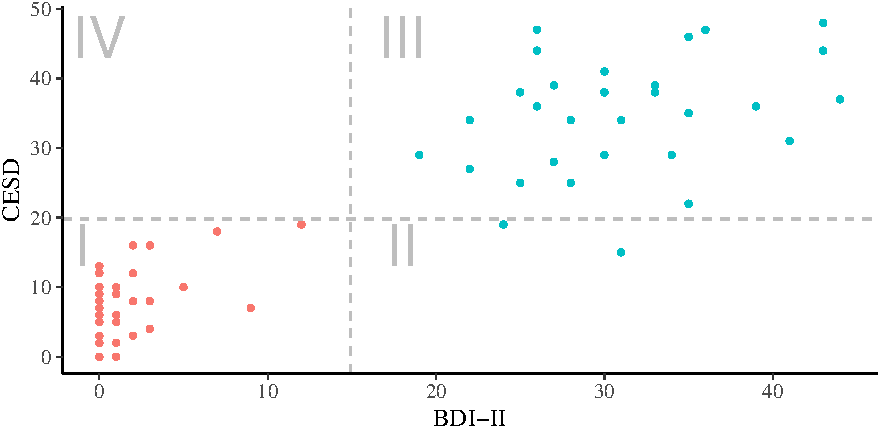
\includegraphics[width=0.8\linewidth]{013_eda_files/figure-latex/zetsche-scatter-1} 

}

\caption{Associazione tra le variabili BDI-II e CES-D nello studio di Zetsche et al. (2019). In arancione sono rappresentate le osservazioni del gruppo di controllo; in azzurro quelle dei pazienti.}\label{fig:zetsche-scatter}
\end{figure}

Dalla figura~\ref{fig:zetsche-scatter} possiamo vedere che i dati mostrano una tendenza a disporsi attorno ad una retta -- nel gergo statistico, questo fatto viene espresso dicendo che i punteggi CES-Dtendono ad essere linearmente associati ai punteggi BDI-II. È ovvio, tuttavia, che tale relazione lineare è lungi dall'essere perfetta -- se fosse perfetta, tutti i punti del diagramma a dispersione si disporrebbero esattamente lungo una retta.

\hypertarget{covarianza}{%
\subsection{Covarianza}\label{covarianza}}

Il problema che ci poniamo è quello di trovare un indice numerico che
descriva di quanto la nube di punti si discosta da una perfetta
relazione lineare tra le due variabili. Per risolvere tale problema
dobbiamo specificare un indice statistico che descriva la direzione e la
forza della relazione lineare tra le due variabili. Ci sono vari indici
statistici che possiamo utilizzare a questo scopo.

Iniziamo a considerare il più importante di tali indici, chiamato
\emph{covarianza}. In realtà la definizione di questo indice non ci
sorprenderà più di tanto in quanto, in una forma solo apparentemente
diversa, l'abbiamo già incontrato in precedenza. Ci ricordiamo infatti
che la varianza di una generica variabile \(X\) è definita come la media
degli scarti quadratici di ciascuna osservazione dalla media:
\begin{equation}
S_{XX} = \frac{1}{n} \sum_{i=1}^n(X_i - \bar{X}) (X_i - \bar{X}).
\label{eq:variance2}
\end{equation}
Infatti, la varianza viene talvolta descritta come la ``covarianza di una
variabile con sé stessa''.

Adesso facciamo un passo ulteriore. Invece di valutare la dispersione di
una sola variabile, chiediamoci come due variabili \(X\) e \(Y\) ``variano
insieme'' (co-variano). È facile capire come una risposta a tale domanda
possa essere fornita da una semplice trasformazione della formula
precedente che diventa:
\begin{equation}
S_{XY} = \frac{1}{n} \sum_{i=1}^n(X_i - \bar{X}) (Y_i - \bar{Y}).
\label{eq:covariance}
\end{equation}
L'eq.~\eqref{eq:covariance} ci fornisce dunque la definizione della covarianza.

Per capire il significato dell'eq.~\eqref{eq:covariance}, supponiamo di dividere il grafico della figura~\ref{fig:zetsche-scatter} in quattro quadranti definiti da una retta verticale passante per la media dei valori BDI-II e da una retta orizzontale passante per la media dei valori CES-D. Numeriamo i quadranti partendo da quello in basso a sinistra e muovendoci in senso antiorario.

Se prevalgono punti nel I e III quadrante, allora la nuvola di punti
avrà un andamento crescente (per cui a valori bassi di \(X\) tendono ad
associarsi valori bassi di \(Y\) e a valori elevati di \(X\) tendono ad
associarsi valori elevati di \(Y\)) e la covarianza segno positivo. Mentre
se prevalgono punti nel II e IV quadrante la nuvola di punti avrà un
andamento decrescente (per cui a valori bassi di \(X\) tendono ad
associarsi valori elevati di \(Y\) e a valori elevati di \(X\) tendono ad
associarsi valori bassi di \(Y\)) e la covarianza segno negativo. Dunque,
il segno della covarianza ci informa sulla direzione della relazione
lineare tra due variabili: l'associazione lineare si dice positiva se la
covarianza è positiva, negativa se la covarianza è negativa.

Il segno della covarianza ci informa sulla direzione della relazione, ma
invece il valore assoluto della covarianza ci dice ben poco. Esso,
infatti, dipende dall'unità di misura delle variabili. Nel caso presente
questo concetto è difficile da comprendere, dato che le due variabili in
esame non hanno un'unità di misura (ovvero, hanno un'unità di misura
arbitraria e priva di significato). Ma quest'idea diventa chiara se
pensiamo alla relazione lineare tra l'altezza e il peso delle persone,
ad esempio. La covarianza tra queste due quantità è certamente positiva,
ma il valore assoluto della covarianza diventa più grande se l'altezza
viene misurata in millimetri e il peso in grammi, e diventa più piccolo
l'altezza viene misurata in metri e il peso in chilogrammi. Dunque, il
valore della covarianza cambia al mutare dell'unità di misura delle
variabili anche se l'associazione tra le variabili resta costante.

\hypertarget{correlazione}{%
\subsection{Correlazione}\label{correlazione}}

Dato che il valore assoluto della covarianza è di difficile
interpretazione -- in pratica, non viene mai interpretato -- è
necessario trasformare la covarianza in modo tale da renderla immune
alle trasformazioni dell'unità di misura delle variabili. Questa
operazione si dice \emph{standardizzazione} e corrisponde alla divisione
della covarianza per le deviazioni standard (\(s_X\), \(s_Y\)) delle due
variabili:

\begin{equation}
r_{XY} = \frac{S_{XY}}{s_X s_Y}.
\label{eq:correlation}
\end{equation}
La quantià che si ottiene in questo modo viene chiamata \emph{correlazione} di Bravais-Pearson (dal nome degli autori che, indipendentemente l'uno dall'altro, la hanno introdotta).

Il coefficiente di correlazione ha le seguenti proprietà:

\begin{itemize}
\tightlist
\item
  ha lo stesso segno della covarianza, dato che si ottiene dividendo
  la covarianza per due numeri positivi;
\item
  è un numero puro, cioè non dipende dall'unità di misura delle
  variabili;
\item
  assume valori compresi tra -1 e +1.
\end{itemize}

Ad esso possiamo assegnare la seguente interpretazione:

\begin{enumerate}
\def\labelenumi{\arabic{enumi}.}
\tightlist
\item
  \(r_{XY} = -1\) \(\rightarrow\) perfetta relazione negativa: tutti i
  punti si trovano esattamente su una retta con pendenza negativa (dal
  quadrante in alto a sinistra al quadrante in basso a destra);
\item
  \(r_{XY} = +1\) \(\rightarrow\) perfetta relazione positiva: tutti i
  punti si trovano esattamente su una retta con pendenza positiva (dal
  quadrante in basso a sinistra al quadrante in alto a destra);
\item
  \(-1 < r_{XY} < +1\) \(\rightarrow\) presenza di una relazione lineare
  di intensità diversa;
\item
  \(r_{XY} = 0\) \(\rightarrow\) assenza di relazione lineare tra \(X\) e
  \(Y\).
\end{enumerate}

\begin{example}
Per i dati della figura~\ref{fig:zetsche-scatter}, la covarianza è 207.426. Il segno positivo della covarianza ci dice che tra le due variabili c'è un'associazione lineare positiva. Per capire qual è l'intensità della relazione lineare tra le due variabili calcoliamo la correlazione.
Essendo le deviazioni standard del BDI-II e del CES-D rispettavamente uguali a 15.37 e 14.93, la correlazione diventa uguale a \(\frac{207.426}{15.38 \cdot 14.93} = 0.904.\) Tale valore è prossimo a 1.0, il che vuol dire che i punti del diagramma a dispersione non si discostano troppo da una retta con una pendenza positiva.
\end{example}

\hypertarget{correlazione-e-causazione}{%
\section{Correlazione e causazione}\label{correlazione-e-causazione}}

Facendo riferimento nuovamente alla figura~\ref{fig:zetsche-scatter}, possiamo dire che, in molte applicazioni (ma non nel caso presente!) l'asse \(x\) rappresenta una quantità nota come \emph{variabile indipendente} e l'interesse si concentra sulla sua influenza sulla \emph{variabile dipendente} tracciata sull'asse \(y\). Ciò presuppone però che sia nota la direzione in cui l'influenza causale potrebbe risiedere. È importante tenere bene a mente che la correlazione è soltanto un indice descrittivo della relazione lineare tra due variabili e in nessun caso può essere usata per inferire alcunché sulle relazioni \textbf{causali} che legano le variabili. È ben nota l'espressione: ``correlazione non significa causazione''.

Di opinione diversa era invece Karl Pearson (1911), il quale ha affermato:

\begin{quote}
Quanto spesso, quando è stato osservato un nuovo fenomeno,
sentiamo che viene posta la domanda: `qual è la sua causa?'. Questa è
una domanda a cui potrebbe essere assolutamente impossibile rispondere.
Invece, può essere più facile rispondere alla domanda: `in che misura
altri fenomeni sono associati con esso?'. Dalla risposta a questa
seconda domanda possono risultare molte preziose conoscenze.
\end{quote}

Che alla seconda domanda posta da Pearson sia facile rispondere è indubbio. Che la nostra comprensione di un fenomeno possa aumentare sulla base delle
informazioni fornite unicamente dalle correlazioni, invece, è molto dubbio e quasi certamente falso.

\hypertarget{usi-della-correlazione}{%
\subsection{Usi della correlazione}\label{usi-della-correlazione}}

Anche se non può essere usata per studiare le relazioni causali, la
correlazione viene usata per molti altri scopi tra i quali, per esempio,
quello di misurare la \emph{validità concorrente} di un test psiologico. Se
un test psicologico misura effettivamente ciò che ci si aspetta che
misuri (nel caso dell'esempio presente, la depressione), allora dovremo
aspettarci che fornisca una correlazione alta con risultati di altri
test che misurano lo stesso costrutto -- come nel caso dei dati di
\autocite{zetschefuture2019}. Un'altra proprietà desiderabile di un test
psicometrico è la \emph{validità divergente}: i risultati di test
psicometrici che misurano costrutti diversi dovrebbero essere poco
associati tra loro. In altre parole, in questo secondo caso dovremmo
aspettarci che la correlazione sia bassa.

\hypertarget{correlazione-di-spearman}{%
\subsection{Correlazione di Spearman}\label{correlazione-di-spearman}}

Una misura alternativa della relazione lineare tra due variabili è
fornita dal coefficiente di correlazione di Spearman e dipende soltanto
dalla relazione d'ordine dei dati, non dagli specifici valori dei dati.
Tale misura di associazione è appropriata quando, del fenomeno in esame,
gli psicologi sono stati in grado di misurare soltanto le relazioni
d'ordine tra le diverse modalità della risposta dei soggetti, non
l'intensità della risposta. Le variabili psicologiche che hanno questa
proprietà si dicono \emph{ordinali}. Nel caso di variabili ordinali, non è
possibile sintetizzare i dati mediante le statistiche descrittive che
abbiamo introdotto in questo capitolo, quali ad esempio la media e la
varianza, ma è invece solo possibile riassumere i dati mediante una
distribuzione di frequenze per le varie modalità della risposta.

\hypertarget{correlazione-nulla}{%
\subsection{Correlazione nulla}\label{correlazione-nulla}}

Un ultimo aspetto da mettere in evidenza a proposito della correlazione riguarda il fatto che la correlazione descrive la direzione e l'intensità della relazione lineare tra due variabili. Relazioni non lineari tra le variabili, anche se sono molto forti, non vengono catturate dalla correlazione. È importante rendersi conto che una correlazione pari a zero non significa che non c'è relazione tra le due variabili, ma solo che tra esse non c'è una relazione \emph{lineare}.

\begin{example}

Un esempio di correlazione nulla in presenza di una chiara relazione (non lineare) tra le variabili è fornito dalla figura~\ref{fig:zerocorr}.

\begin{Shaded}
\begin{Highlighting}[]
\FunctionTok{library}\NormalTok{(}\StringTok{"datasauRus"}\NormalTok{)}
\NormalTok{slant }\OtherTok{\textless{}{-}} \FunctionTok{ggplot}\NormalTok{(}
\NormalTok{  datasaurus\_dozen\_wide,}
  \FunctionTok{aes}\NormalTok{(}\AttributeTok{x =}\NormalTok{ slant\_down\_x, }\AttributeTok{y =}\NormalTok{ slant\_down\_y),}
  \AttributeTok{colour =}\NormalTok{ dataset}
\NormalTok{)}
\NormalTok{slant }\OtherTok{\textless{}{-}}\NormalTok{ slant }\SpecialCharTok{+}
  \FunctionTok{geom\_point}\NormalTok{()}
\NormalTok{slant }\OtherTok{\textless{}{-}}\NormalTok{ slant }\SpecialCharTok{+}
  \FunctionTok{theme\_void}\NormalTok{()}
\NormalTok{slant }\OtherTok{\textless{}{-}}\NormalTok{ slant }\SpecialCharTok{+}
  \FunctionTok{theme}\NormalTok{(}
    \AttributeTok{legend.position =} \StringTok{"none"}\NormalTok{,}
    \AttributeTok{panel.border =} \FunctionTok{element\_rect}\NormalTok{(}\AttributeTok{colour =} \StringTok{"black"}\NormalTok{, }\AttributeTok{fill =} \ConstantTok{NA}\NormalTok{, }\AttributeTok{size =} \DecValTok{1}\NormalTok{),}
    \AttributeTok{plot.margin =} \FunctionTok{margin}\NormalTok{(}\DecValTok{0}\NormalTok{, }\DecValTok{2}\NormalTok{, }\DecValTok{0}\NormalTok{, }\DecValTok{2}\NormalTok{), }\AttributeTok{aspect.ratio =} \DecValTok{1}
\NormalTok{  )}

\NormalTok{dino }\OtherTok{\textless{}{-}} \FunctionTok{ggplot}\NormalTok{(}
\NormalTok{  datasaurus\_dozen\_wide,}
  \FunctionTok{aes}\NormalTok{(}\AttributeTok{x =}\NormalTok{ dino\_x, }\AttributeTok{y =}\NormalTok{ dino\_y),}
  \AttributeTok{colour =}\NormalTok{ dataset}
\NormalTok{) }\SpecialCharTok{+}
  \FunctionTok{geom\_point}\NormalTok{()}

\NormalTok{dino }\OtherTok{\textless{}{-}}\NormalTok{ dino }\SpecialCharTok{+}
  \FunctionTok{theme\_void}\NormalTok{()}
\NormalTok{dino }\OtherTok{\textless{}{-}}\NormalTok{ dino }\SpecialCharTok{+}
  \FunctionTok{theme}\NormalTok{(}
    \AttributeTok{legend.position =} \StringTok{"none"}\NormalTok{,}
    \AttributeTok{panel.border =} \FunctionTok{element\_rect}\NormalTok{(}\AttributeTok{colour =} \StringTok{"black"}\NormalTok{, }\AttributeTok{fill =} \ConstantTok{NA}\NormalTok{, }\AttributeTok{size =} \DecValTok{1}\NormalTok{),}
    \AttributeTok{plot.margin =} \FunctionTok{margin}\NormalTok{(}\DecValTok{0}\NormalTok{, }\DecValTok{2}\NormalTok{, }\DecValTok{0}\NormalTok{, }\DecValTok{2}\NormalTok{), }\AttributeTok{aspect.ratio =} \DecValTok{1}
\NormalTok{  )}

\NormalTok{slant }\SpecialCharTok{+}\NormalTok{ dino}
\end{Highlighting}
\end{Shaded}

\begin{figure}[h]

{\centering 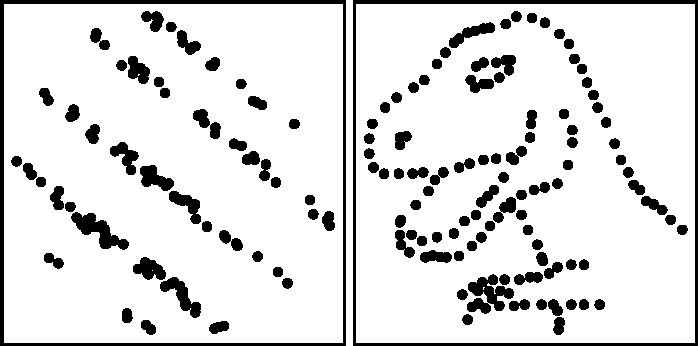
\includegraphics[width=0.8\linewidth]{013_eda_files/figure-latex/zerocorr-1} 

}

\caption{Due insiemi di dati (fittizi) per i quali i coefficienti di correlazione di Pearson sono entrambi 0. Ma questo non significa che non vi sia alcuna relazione tra le variabili.}\label{fig:zerocorr}
\end{figure}

\end{example}

\hypertarget{considerazioni-conclusive}{%
\section*{Considerazioni conclusive}\label{considerazioni-conclusive}}
\addcontentsline{toc}{section}{Considerazioni conclusive}

La prima fase dell'analisi dei dati ci porta a riassumere i dati mediante gli strumenti della statistica descrittiva.
Le tipiche domande che vengono affrontate in questa fase sono: qual è la
distribuzione delle variabili di interesse? Quali relazioni a coppie si
possono osservare nel campione? Ci sono delle osservazioni `anomale',
ovvero estremamente discrepanti rispetto alle altre, sia quando si
esaminano le statistiche descrittive univariate (ovvero, quelle che
riguardano le caratteristiche di una variabile presa singolarmente), sia
quando vengono esaminate le statistiche bivariate (ovvero, le
statistiche che descrivono l'associazione tra le variabili)? È
importante avere ben chiare le idee su questi punti prima di procedere
con qualsiasi procedura statistica di tipo inferenziale. Per rispondere
alle domande che abbiamo elencato sopra, ed ad altre simili, è molto
utile procedere con delle rappresentazioni grafiche dei dati. È chiaro che, quando disponiamo di grandi moli di dati (come è sempre il caso in psicologia), le operazioni descritte sopra devono essere svolte mediante un software statistico.


% Bibliography
%%%%%%%%%%%%%%%%%%%%%%%%%%%%%%%%%%%%%%%%%%%%%%%%%%%%%%%%%%

\backmatter
\SmallMargins

\printbibliography
\onecolumn


% Tables (of tables, of figures)
%%%%%%%%%%%%%%%%%%%%%%%%%%%%%%%%%%%%%%%%%%%%%%%%%%%%%%%%%%


\cleardoublepage
\LargeMargins
\listoffigures


% After-body (LaTeX code inclusion)
%%%%%%%%%%%%%%%%%%%%%%%%%%%%%%%%%%%%%%%%%%%%%%%%%%%%%%%%%%




% Back cover
%%%%%%%%%%%%%%%%%%%%%%%%%%%%%%%%%%%%%%%%%%%%%%%%%%%%%%%%%%%

% Even page, small margins, no running head, no page number.
\evenpage
\SmallMargins
\thispagestyle{empty}

\begin{normalsize}

\begin{description}

\selectlanguage{italian}
\item[Abstract]
This document contains the material of the lessons of Psicometria B000286 (2021/2022) aimed at students of the first year of the Degree Course in Psychological Sciences and Techniques of the University of Florence, Italy.
\item[Keywords]
Data science, Bayesian statistics.
~\\

\end{description}

\end{normalsize}


\end{document}
